\documentclass[xcolor=dvipsnames,serif,10pt]{beamer}
\usepackage{etex}

\usepackage{beamerthemesplit}
\usepackage{graphics}
\usepackage{graphicx}
\usepackage{hyperref}
\usepackage[normalem]{ulem}
%\usefonttheme{professionalfonts}
%\usepackage{times}
\usepackage{rotating}
\usepackage{tikz}
\usepackage{amsmath,cancel}
\usepackage{mathtools}
\usepackage{verbatim}
\usetikzlibrary{arrows,shapes}
\usepackage{listings}
\usepackage[]{geometry}
\usepackage{ifxetex}
\ifxetex{%
  \usepackage{fontspec}
  \setmainfont{Linux Libertine O} % or any font on your system
  \newfontfamily\quotefont[Ligatures=TeX]{Linux Libertine O} % or any font on your system
\else
  \usepackage[T1]{fontenc}
  \usepackage{libertine} % or any other font package (or none)
  \newcommand*\quotefont{\fontfamily{fxl}} % selects Libertine for quote font
\fi
\usepackage{framed}

\usepackage{soul}
\usetikzlibrary{calc}
\usetikzlibrary{decorations.pathmorphing}
\usetikzlibrary{decorations.text}
\usetikzlibrary{calc,shapes.callouts,shapes.arrows}
\makeatletter

\newcommand{\defhighlighter}[3][]{%
  \tikzset{every highlighter/.style={color=#2, fill opacity=#3, #1}}%
}

\defhighlighter{yellow}{.5}

\newcommand{\highlight@DoHighlight}{
  \fill [ decoration = {random steps, amplitude=1pt, segment length=15pt}
        , outer sep = -15pt, inner sep = 0pt, decorate
        , every highlighter, this highlighter ]
        ($(begin highlight)+(0,8pt)$) rectangle ($(end highlight)+(0,-3pt)$) ;
}

\newcommand{\highlight@BeginHighlight}{
  \coordinate (begin highlight) at (0,0) ;
}

\newcommand{\highlight@EndHighlight}{
  \coordinate (end highlight) at (0,0) ;
}

\newdimen\highlight@previous
\newdimen\highlight@current

\DeclareRobustCommand*\highlight[1][]{%
  \tikzset{this highlighter/.style={#1}}%
  \SOUL@setup
  %
  \def\SOUL@preamble{%
    \begin{tikzpicture}[overlay, remember picture]
      \highlight@BeginHighlight
      \highlight@EndHighlight
    \end{tikzpicture}%
  }%
  %
  \def\SOUL@postamble{%
    \begin{tikzpicture}[overlay, remember picture]
      \highlight@EndHighlight
      \highlight@DoHighlight
    \end{tikzpicture}%
  }%
  %
  \def\SOUL@everyhyphen{%
    \discretionary{%
      \SOUL@setkern\SOUL@hyphkern
      \SOUL@sethyphenchar
      \tikz[overlay, remember picture] \highlight@EndHighlight ;%
    }{%
    }{%
      \SOUL@setkern\SOUL@charkern
    }%
  }%
  %
  \def\SOUL@everyexhyphen##1{%
    \SOUL@setkern\SOUL@hyphkern
    \hbox{##1}%
    \discretionary{%
      \tikz[overlay, remember picture] \highlight@EndHighlight ;%
    }{%
    }{%
      \SOUL@setkern\SOUL@charkern
    }%
  }%
  %
  \def\SOUL@everysyllable{%
    \begin{tikzpicture}[overlay, remember picture]
      \path let \p0 = (begin highlight), \p1 = (0,0) in \pgfextra
        \global\highlight@previous=\y0
        \global\highlight@current =\y1
      \endpgfextra (0,0) ;
      \ifdim\highlight@current < \highlight@previous
        \highlight@DoHighlight
        \highlight@BeginHighlight
      \fi
    \end{tikzpicture}%
    \the\SOUL@syllable
    \tikz[overlay, remember picture] \highlight@EndHighlight ;%
  }%
  \SOUL@
}
\makeatother


% wrap everything in its own environment
\newenvironment{shadequote}%
{\begin{quote}\openquote}
{\hfill\closequote\end{quote}}

\newcommand{\arrowthis}[2]{
        \tikz[remember picture,baseline]{\node[anchor=base,inner sep=0,outer sep=0]%
        (#1) {\underline{#1}};
        \node[overlay,single arrow,draw=none,fill=red!50,anchor=tip,rotate=60] 
        at (#1.south) {#2};}%
    }%

\newcommand{\speechthis}[2]{
        \tikz[remember picture,baseline]{\node[anchor=base,inner sep=0,outer sep=0]%
        (#1) {\underline{#1}};\node[overlay,ellipse callout,fill=blue!50] 
        at ($(#1.north)+(-.5cm,0.8cm)$) {#2};}%
    }%

\newcommand{\bubblethis}[2]{
        \tikz[remember picture,baseline]{\node[anchor=base,inner sep=0,outer sep=0]%
        (#1) {\underline{#1}};\node[overlay,cloud callout,callout relative pointer={(0.2cm,-0.7cm)},%
        aspect=2.5,fill=yellow!90] at ($(#1.north)+(-0.5cm,1.6cm)$) {#2};}%
    }%

\newcommand{\pointthis}[2]{
        \tikz[remember picture,baseline]{\node[anchor=base,inner sep=0,outer sep=0]%
        (#1) {\underline{#1}};\node[overlay,rectangle callout,%
        callout relative pointer={(0.2cm,0.7cm)},fill=green!50] at ($(#1.north)+(-.5cm,-1.4cm)$) {#2};}%
        }%


\usetikzlibrary{mindmap,backgrounds}

    \definecolor{listcomment}{rgb}{0.0,0.5,0.0}
    \definecolor{listkeyword}{rgb}{0.0,0.0,0.5}
    \definecolor{listnumbers}{gray}{0.65}
    \definecolor{listlightgray}{gray}{0.9}
    \definecolor{listwhite}{gray}{1.0}


\usetheme[secheader]{Boadilla}
\useoutertheme{miniframes}
\useinnertheme{circles}
\usecolortheme{myct}
\usepackage[latin1]{inputenc}

\graphicspath{{Figures/}{../Figures/}}

\setlength{\tabcolsep}{1pt}

\newcommand\fontvi{\fontsize{6}{8}\selectfont}
\newcommand{\ColIndent}{\hspace{\labelwidth}\hspace{\labelsep}\hspace{\labelsep}\hspace{\labelsep}\hspace{\labelsep}}

\usetikzlibrary{backgrounds}
\usetikzlibrary{positioning}
\makeatletter


%%%%%%%%%%%%%%%%%%%%%%%%%%%%%
%%  Title slide
%%%%%%%%%%%%%%%%%%%%%%%%%%%%%

\title[The ANTs Cortical Thickness Pipeline]{The ANTs Cortical Thickness Pipeline}
\author[N. Tustison]{%
  N.J. Tustison$^{1}$, B.B. Avants$^{2}$, P.A. Cook$^{2}$, G. Song$^{2}$, S. Das$^{2}$, N. van Strien$^{3}$, J.R. Stone$^{1}$, J.C. Gee$^{2}$
  }
\date[SPIE 2013:  Orlando, FL]{}
\institute[ntustison@virginia.edu]{
  $^{1}$Department of Radiology and Medical Imaging, University of Virginia \\
  $^{2}$Penn Image and Computing Science Laboratory, University of Pennsylvania \\
  $^{3}$Department of Circulation and Medical Imaging, Norwegian University of Science and Technology}

%\pgfdeclaremask{fsu}{fsu_logo_ybkgrd}
%\pgfdeclareimage[width=1cm]{logo}{ants_logo}
%\logo{\vbox{\vskip0.1cm\hbox{\pgfuseimage{logo}}}}

%\logo{
%  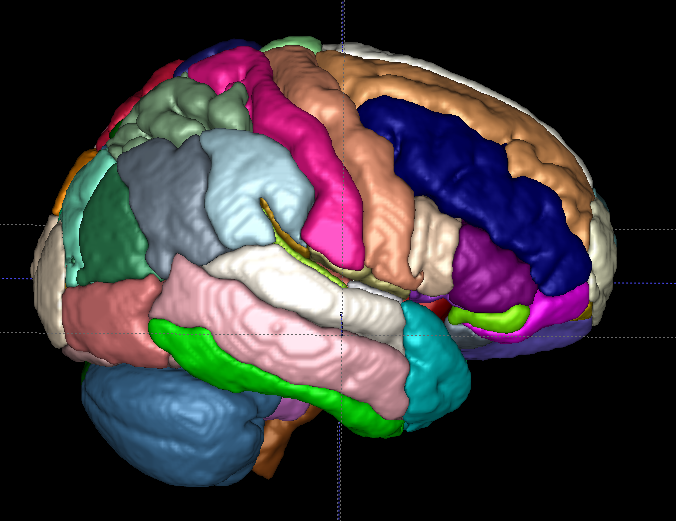
\includegraphics[height=0.8cm]{brain2.png}
%  
\includegraphics[height=0.8cm]{itkLogo.jpg}
%  }

\begin{document}

\tikzstyle{every picture}+=[remember picture]

\frame{\titlepage}

%%%%%%%%%%%%%%%%%%%%%%%%%%%%%
%%  Cortical thickness uses
%%%%%%%%%%%%%%%%%%%%%%%%%%%%%

\begin{frame}{Cortical thickness studies}
\begin{columns}[c]
  \begin{column}{0.45\textwidth}
    \begin{itemize}
    \item Huntington's disease
    \item schizophrenia
    \item bipolar disorder
    \item Alzheimer's disease
    \item Fronto-temporal dementia
    \item Parkinson's disease
    \item Williams syndrome
    \item multiple sclerosis
    \item autism
    \item migraines
    \item chronic smoking
    \end{itemize}
  \end{column}  
  \begin{column}{0.45\textwidth}
    \begin{itemize}
    \item alcholism
    \item cocaine addiction
    \item Tourette syndrome in children
    \item scoliosis in female adolescents
    \item obsessive compulsive disorder
    \item attention deficit hyperactivity disorder
    \item obesity
    \item heritable depression
    \item elderly depression
    \end{itemize}
  \end{column}  
\end{columns}
\end{frame}

%%%%%%%%%%%%%%%%%%%%%%%%%%%%%
%%  Cortical thickness uses 2
%%%%%%%%%%%%%%%%%%%%%%%%%%%%%

\begin{frame}{Cortical thickness studies (cont.)}
\begin{columns}[c]
  \begin{column}[t]{0.45\textwidth}
    \begin{itemize}
    \item Correlated with:
      \begin{itemize}
		    \item age
		    \item gender
		    \item untreated transsexuality
		    \item handedness
		    \item intelligence
		    \item athletic ability
		    \item musical ability
		    \item tendency towards criminality
		    \item Tetris-playing ability in female adolescents
		  \end{itemize}    
    \end{itemize}
  \end{column}  
  \begin{column}[t]{0.45\textwidth}
    \begin{itemize}
     \item functional connectivity relationships
    \end{itemize}
  \end{column}  
\end{columns}
\end{frame}

%%%%%%%%%%%%%%%%%%%%%%%%%%%%%
%%  Motivation
%%%%%%%%%%%%%%%%%%%%%%%%%%%%%

% Mention having a complete volumetric pipeline analogous to
% the entire Freesurfer pipeline.  Also talk about Clarkson's
% paper.


\begin{frame}{}

  \begin{center}
    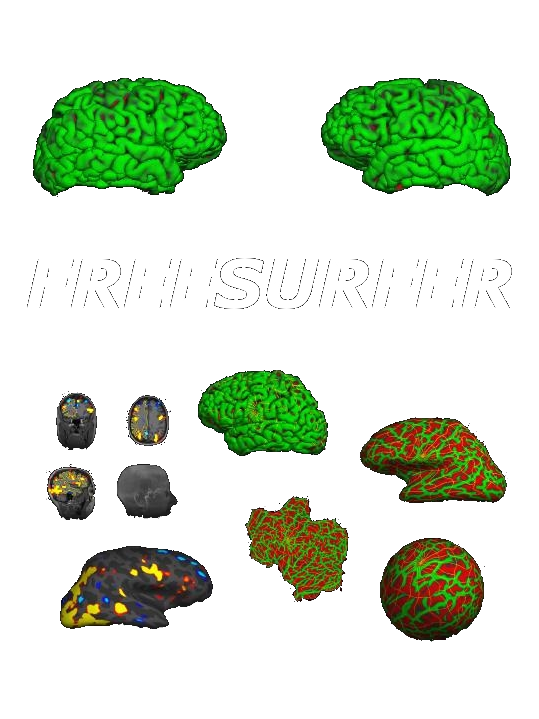
\includegraphics[height=8cm]{Freesurfer.png}
   \end{center}

\end{frame}


%%%%%%%%%%%%%%%%%%%%%%%%%%%%%
%%  Materials
%%%%%%%%%%%%%%%%%%%%%%%%%%%%%

\begin{frame}{Data}
\begin{columns}[c]
  \begin{column}[c]{0.4\textwidth}
      \begin{itemize}
		    \item IXI (Imperial College)
		      \begin{itemize}
		        \item 581 subjects
		        \item T1, T2, PD, DWI
		        \item 3 sites, 1.5 \& 3 T
		      \end{itemize}
		    \item Oasis (WUSTL)
		      \begin{itemize}
		        \item 416 subjects
		        \item 100 mild AD
		        \item defaced
		      \end{itemize}
		    \item NKI/Rockland
		      \begin{itemize}
		        \item 188 subjects
		        \item T1, T2, R-fMRI, DTI
		        \item defaced
		      \end{itemize}
		    \item Kirby (VU)
		      \begin{itemize}
		        \item 41 subjects
		        \item T1, T2, DTI,\ldots
		      \end{itemize}
		  \end{itemize}    
  \end{column}  
 \begin{column}[c]{0.4\textwidth}
   \begin{tabular}{cc}
     \vspace{-0.05cm}
     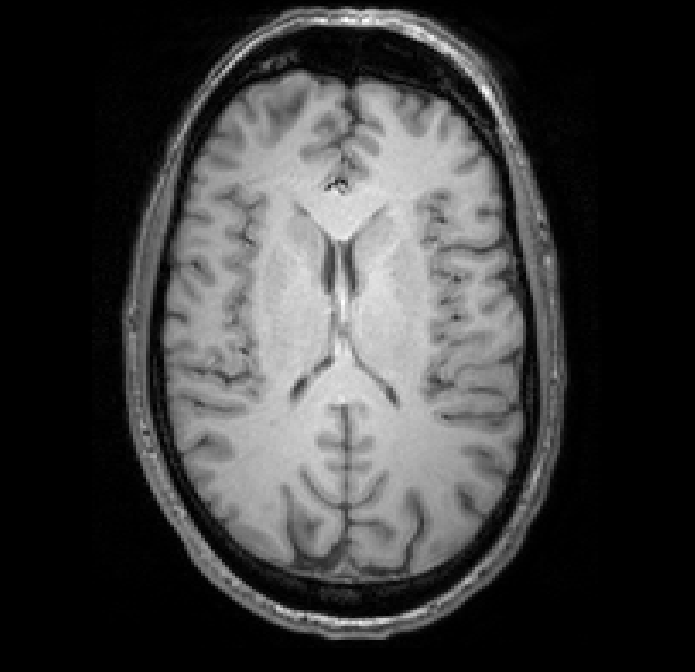
\includegraphics[width=1.75cm]{IXI048_axial.png} &  
     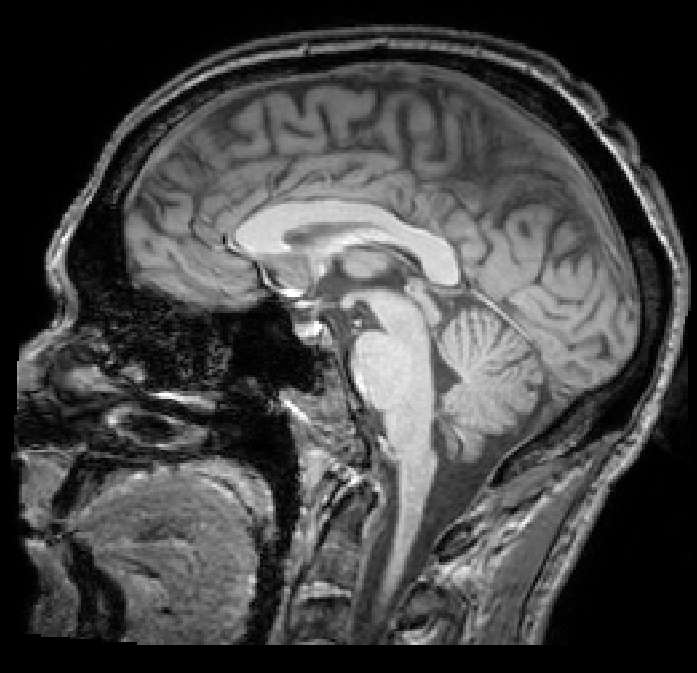
\includegraphics[width=1.75cm]{IXI048_sag.png} \\
     \vspace{-0.05cm}
     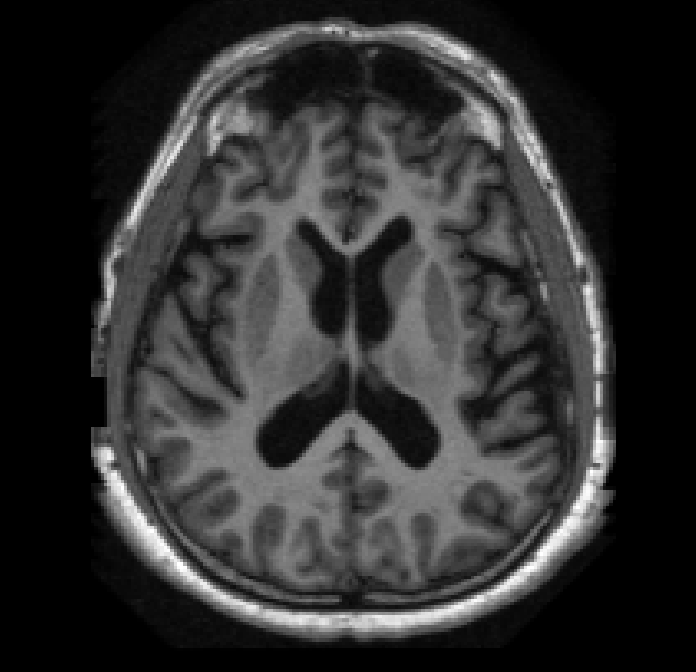
\includegraphics[width=1.75cm]{OAS1_0039_axial.png} &  
     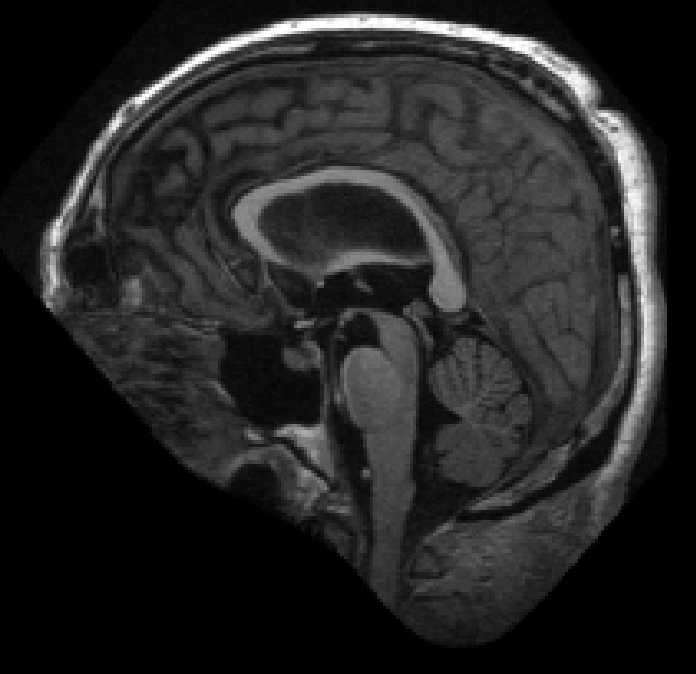
\includegraphics[width=1.75cm]{OAS1_0039_sag.png} \\
     \vspace{-0.05cm}
     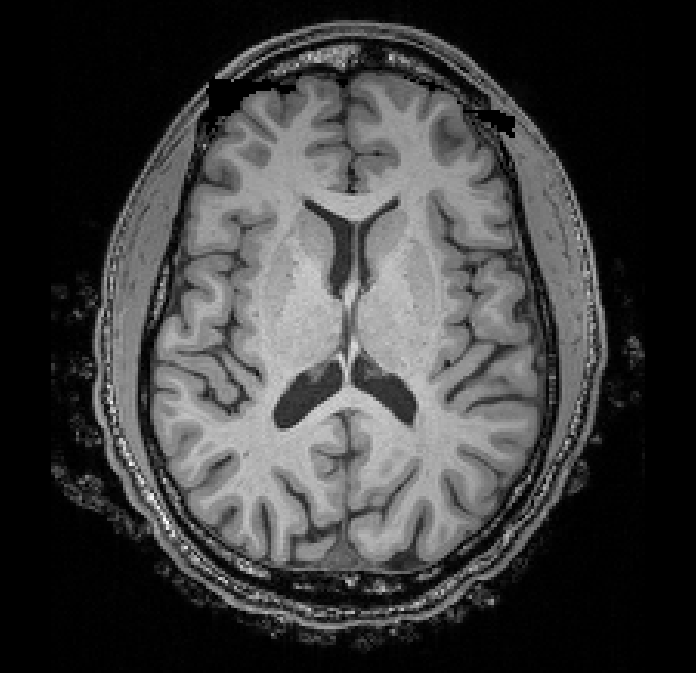
\includegraphics[width=1.75cm]{NKI_2861923_axial.png} &  
     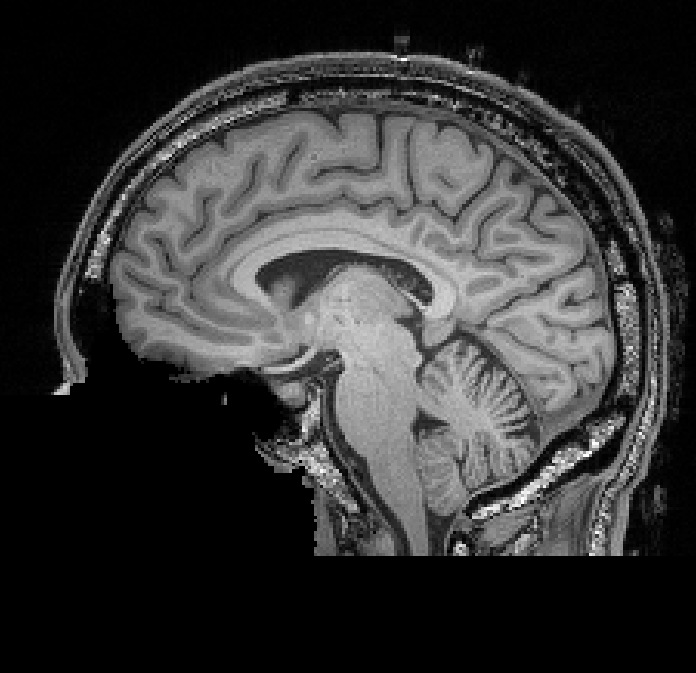
\includegraphics[width=1.75cm]{NKI_2861923_sag.png} \\
     \vspace{-0.05cm}
     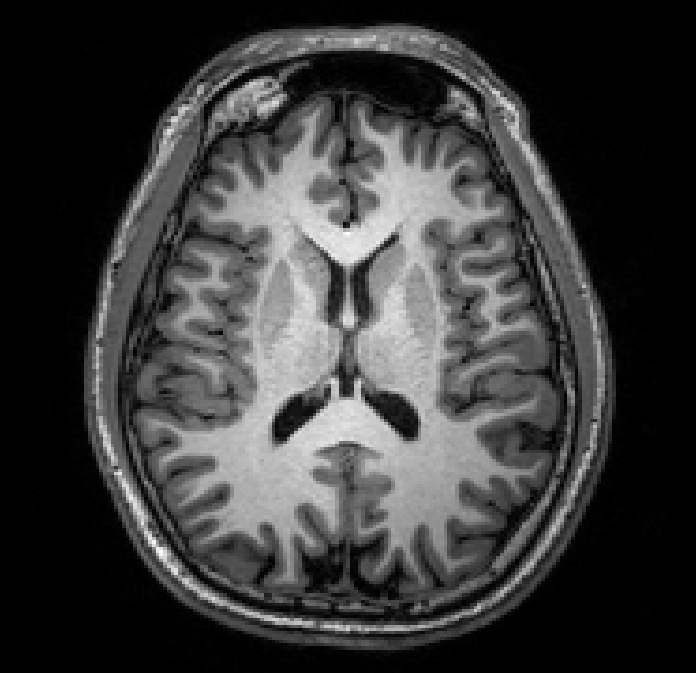
\includegraphics[width=1.75cm]{KKI2009-25_axial.png} &  
     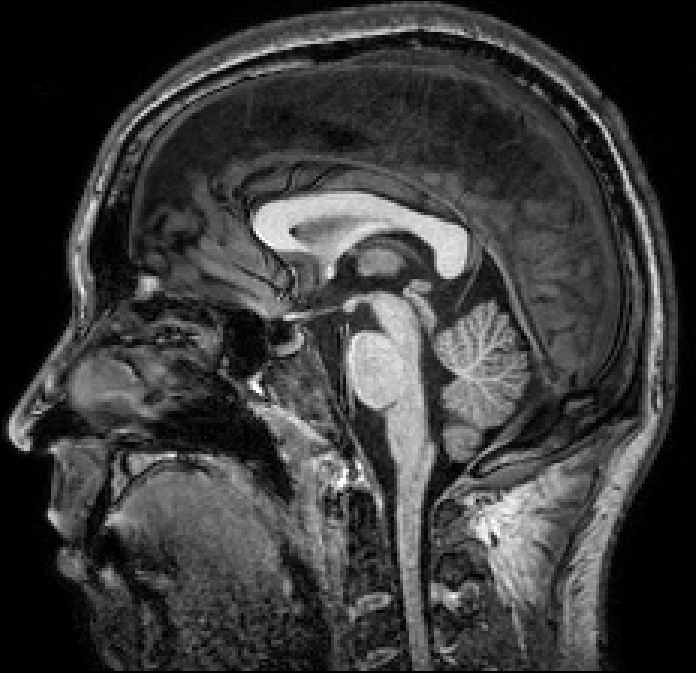
\includegraphics[width=1.75cm]{KKI2009-25_sag.png} 
   \end{tabular}
 \end{column}
\end{columns}

\end{frame}
  
%%%%%%%%%%%%%%%%%%%%%%%%%%%%%
%%  Algorithms
%%%%%%%%%%%%%%%%%%%%%%%%%%%%%

\begin{frame}{Algorithms}

\begin{center}
  \begin{itemize}
    \item \texttt{N4BiasFieldCorrection.cxx}\tikz[remember picture] \node (a) {\vphantom{X}};
    \item \texttt{antsRegistration.cxx}\tikz[remember picture] \node (b) {\vphantom{X}};
    \item \texttt{antsAffineInitializer.cxx}
    \item \texttt{Atropos.cxx}\tikz[remember picture] \node (c) {\vphantom{X}};
    \item \texttt{KellyKapowski.cxx}\tikz[remember picture] \node (d) {\vphantom{X}};
    \item \texttt{ImageMath.cxx}
    \item \texttt{abp.sh}
  \end{itemize}    
\end{center}

\begin{tikzpicture}[remember picture,overlay]
\path<2> (a.east) ++(0,1) node[anchor=west,ellipse callout,fill=red!50,opacity=1, callout absolute pointer={(a.mid)},text =black]  {IEEE-TMI 2010};
\end{tikzpicture}

\begin{tikzpicture}[remember picture,overlay]
\path<3> (b.east) ++(0,1) node[anchor=west,ellipse callout,fill=yellow!50,opacity=1, callout absolute pointer={(b.mid)},text =black]  {MIA 2008, IEEE-TIP 2009};
\end{tikzpicture}

\begin{tikzpicture}[remember picture,overlay]
\path<4> (c.east) ++(0,1) node[anchor=west,ellipse callout,fill=green!50,opacity=1, callout absolute pointer={(c.mid)},text =black]  {Neuroinformatics 2011};
\end{tikzpicture}

\begin{tikzpicture}[remember picture,overlay]
\path<5> (d.east) ++(0,1) node[anchor=west,ellipse callout,fill=orange!50,opacity=1, callout absolute pointer={(d.mid)},text =black]  {Neuroimage 2009};
\end{tikzpicture}

\end{frame}

%%%%%%%%%%%%%%%%%%%%%%%%%%%%%
%%  abp.sh
%%%%%%%%%%%%%%%%%%%%%%%%%%%%%

\lstset{frame = htb,
        framerule = 0.25pt,
        float,
        fontadjust,
        backgroundcolor={\color{black}},
        basicstyle=\fontfamily{pcr}\selectfont\tiny\color{green},
        keywordstyle = {\ttfamily\color{green}\textbf},
        identifierstyle = {\ttfamily},
        commentstyle = {\ttfamily\color{green}\textit},
        stringstyle = {\ttfamily},
        showstringspaces = false,
        showtabs = false
        numbers = none,
        numbersep = 6pt,
        numberstyle={\ttfamily\color{listnumbers}},
        tabsize = 2,
        language=bash,
        floatplacement=!h,
%        caption={Representative script used for the LPBA40 evaluation.},
        captionpos=b,
        label=listing:script
        }

\begin{frame}[fragile]
\frametitle{\texttt{abp.sh}}

\begin{lstlisting}
$ sh ~/Pkg/Utilities/scripts/abp.sh 

This script, apb.sh, performs T1 anatomical brain processing where the following
steps are currently applied:

  1. Brain extraction
  2. Brain 3-tissue segmentation
  3. Cortical thickness
  4. (Optional) registration to a template

Usage:

abp.sh -d imageDimension
       -a anatomicalImage.nii.gz
       -e brainExtractionTemplate
       -m brainExtractionProbabilityMask
       -l brainSegmentationTemplate
       -p brainSegmentationPriors
       <OPTARGS>
       -o outputPrefix

Example:

  bash /Users/ntustison/Pkg/Utilities/scripts/abp.sh -d 3 -i t1.nii.gz -e brainWithSkullTemplate.nii.gz
  -m brainPrior.nii.gz -l segmentationTemplate.nii.gz -p segmentationPriors%d.nii.gz -o output

Required arguments:
   ...

Optional arguments:
   ...

\end{lstlisting}                 

\end{frame}

%%%%%%%%%%%%%%%%%%%%%%%%%%%%%
%%  ANTs pipeline
%%%%%%%%%%%%%%%%%%%%%%%%%%%%%

\begin{frame}{ANTs pipeline for cortical thickness estimation}

\tikzstyle{format} = [draw, thick, fill=middlecolour]
\tikzstyle{format2} = [draw, thin, fill=middlecolour]
\tikzstyle{medium} = [ellipse, draw, thin, fill=green!20, minimum height=2.5em]
\tikzstyle{line} = [-latex',very thick,textcolour]

\usetikzlibrary{calc,decorations.pathmorphing,patterns}
\pgfdeclaredecoration{penciline}{initial}{
    \state{initial}[width=+\pgfdecoratedinputsegmentremainingdistance,
    auto corner on length=1mm,]{
        \pgfpathcurveto%
        {% From
            \pgfqpoint{\pgfdecoratedinputsegmentremainingdistance}
                      {\pgfdecorationsegmentamplitude}
        }
        {%  Control 1
        \pgfmathrand
        \pgfpointadd{\pgfqpoint{\pgfdecoratedinputsegmentremainingdistance}{0pt}}
                    {\pgfqpoint{-\pgfdecorationsegmentaspect
                     \pgfdecoratedinputsegmentremainingdistance}%
                               {\pgfmathresult\pgfdecorationsegmentamplitude}
                    }
        }
        {%TO 
        \pgfpointadd{\pgfpointdecoratedinputsegmentlast}{\pgfpoint{1pt}{1pt}}
        }
    }
    \state{final}{}
}

\begin{center}
\begin{tikzpicture}[node distance=3cm, auto,>=latex', thick,decoration=penciline, decorate]
    % We need to set at bounding box first. Otherwise the diagram
    % will change position for each frame.
    \path[use as bounding box] (-1,0) rectangle (10,0);
    
%\uncover<1->{
    \path[->,rounded corners=0.1cm] node[format, yshift=2cm, text width=1.5cm, text height=0.0cm ] (ixi) { 
        \begin{center}
			  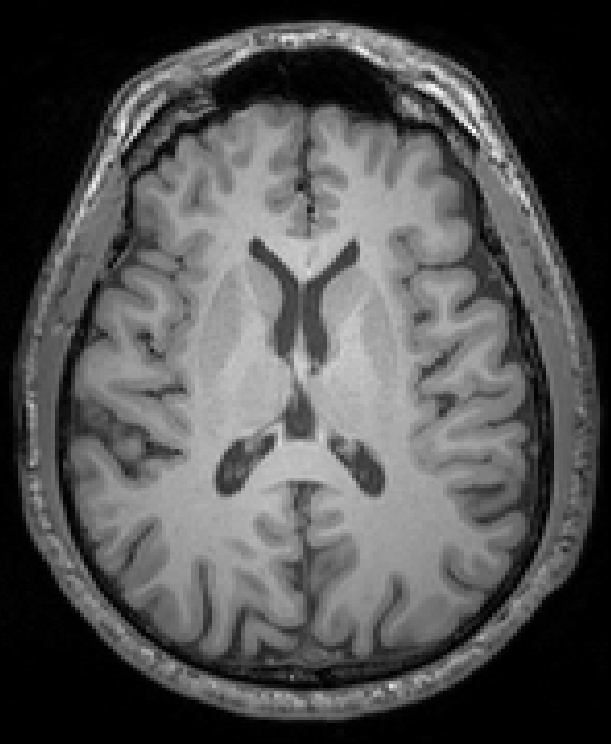
\includegraphics[height=1.75cm]{IXI221.png} \\
        \tiny{Input MRI}
        \end{center}
			  };
    \path[->] node[format, right of=ixi, xshift=0.5cm, text width=1.25cm, text height=-0.35cm ] (n4) {
          \begin{center}
            \tiny{Initial N4 bias correction}
          \end{center}
        };
    \draw[->] (ixi.0) --  (n4.180);    
    \path[->] node[format, below of=n4, yshift = 1.25cm, text width=1.25cm, text height=-0.35cm ] (be) {
          \begin{center}
            \tiny{Brain extraction}
          \end{center}
        };
    \draw[->] (n4.-90) -- (be.90);    
    \path[->] node[format, below of=be, yshift = 1.25cm, text width=1.25cm, text height=-0.35cm ] (n4_2) {
          \begin{center}
            \tiny{N4 using WM estimate}
          \end{center}
        };
    \draw[->] (be.-90) -- (n4_2.90);    
    \path[->] node[format, below of=n4_2, yshift=1.25cm, text width=1.25cm, text height=-0.35cm ] (atropos) {
          \begin{center}
            \tiny{3-tissue segmentation}
          \end{center}
        };
    \draw[->] (n4_2.-90) -- (atropos.90);    
    \path[->] node[diamond, draw, thick, fill=middlecolour, left of=atropos, xshift=1.75cm, yshift=0.875cm, text width=0.5cm, text height=-0.65cm ] (conv) {
          \begin{center}
            \tiny{Conv.?}
          \end{center}
        };
    \draw[->] (atropos.180) -| (conv.270);    
    \draw[->] (conv.90) |- node {\tiny no} (n4_2.180);    
    
    \path[->] node[format, left of=atropos, xshift=-0.5cm, text width=1.5cm, text height=-0.35cm  ] (kk) {
        \begin{center}
        \tiny{Cortical thickness estimation}
        \end{center}
			  };
    \path[->,rounded corners=0.1cm] node[format, above of=kk, yshift=-1cm, text width=1.5cm, text height=-0.3cm  ] (kkmap) {
        \begin{center}
			  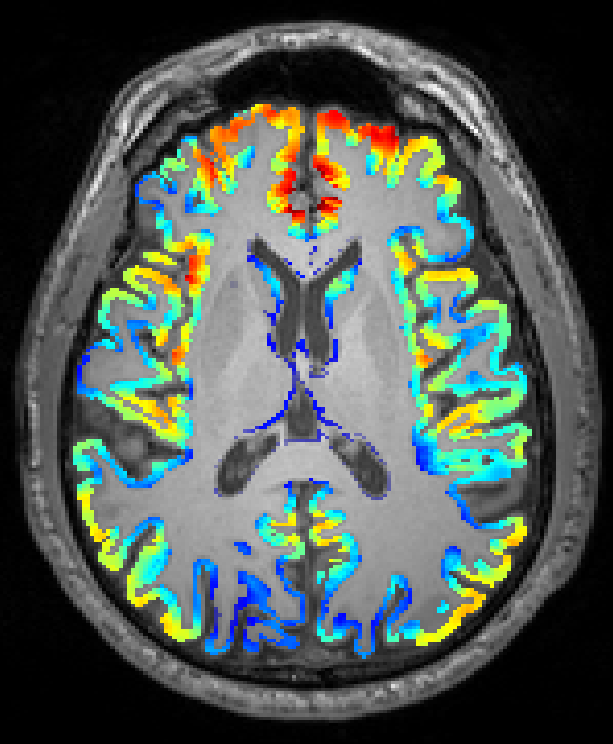
\includegraphics[height=1.75cm]{IXI221_direct.png} \\
        \tiny{Thickness map}
        \end{center}
			  };
			  
    \draw[->] (conv.180) -- node {\tiny yes} ([yshift=0cm,xshift=-0.45cm]conv.180) |- (kk.0);    
    \draw[<-] (kkmap.270) -- (kk.90);    
%}

%\uncover<2->{
    \path[->,rounded corners=0.1cm] 
      node[format, right of=n4, xshift=1.15cm, yshift=-2.5cm,text width=4.75cm,text height=-0.3cm  ] (template) { 
        \begin{center}
        \tiny{Oasis template (35 normals)}
        \begin{tabular}{cc}
          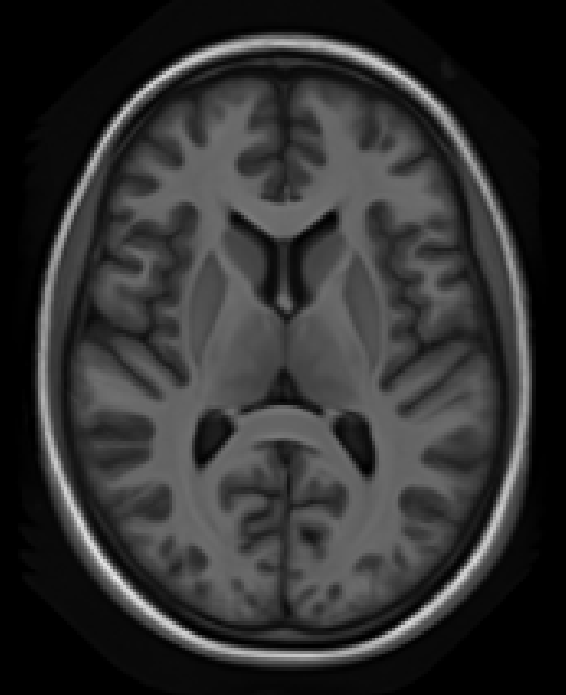
\includegraphics[width=1.5cm]{MICCAI_T1.png} &
          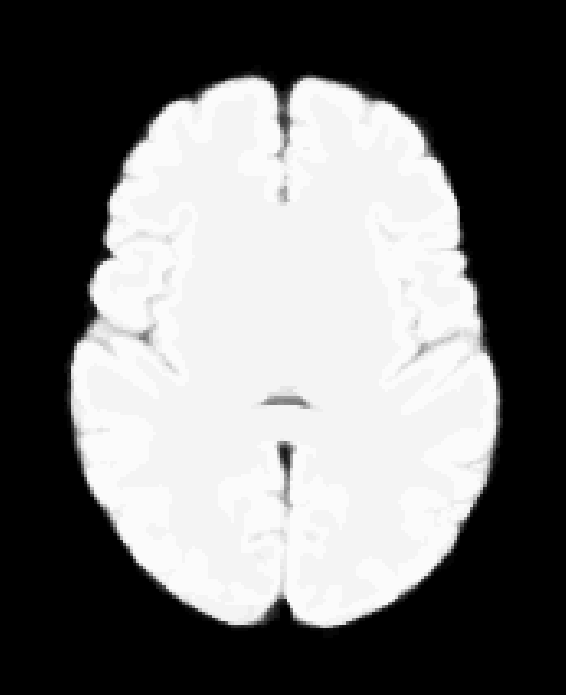
\includegraphics[width=1.5cm]{MICCAI_probMask.png} \\
          \tiny{T1} & \tiny{Whole brain} 
        \end{tabular} \\
        \begin{tabular}{ccc}
          
\includegraphics[width=1.5cm]{MICCAI_probCSF.png} &
          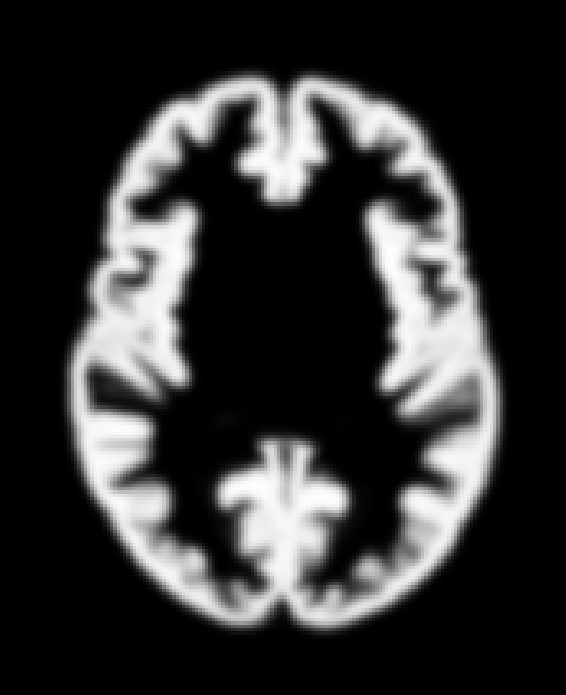
\includegraphics[width=1.5cm]{MICCAI_probGM.png} &
          
\includegraphics[width=1.5cm]{MICCAI_probWM.png} \\
          \tiny{CSF} & \tiny{GM} & \tiny{WM}
        \end{tabular} \\
        \end{center}
			  };
    \draw[->,dashed] (template.160) -- ([yshift=0cm,xshift=-0.5cm]template.160) |- (be.0); 
    \draw[->,dashed] (template.200) -- ([yshift=0cm,xshift=-0.5cm]template.200) |- (atropos.0); 
%}
    
%\uncover<3->{
  \node[decorate,draw,minimum height=7.25cm,minimum width=5.65cm,dashed,rounded corners=0.2cm, thin, color = yellow] (c) at (1.7,-0.35) {};
%}  
%\uncover<4->{
  \node[decorate,draw,minimum height=5.25cm,minimum width=5.55cm,dashed,rounded corners=0.2cm, thin, color = red] (c) at (7.7,-0.45) {};
%}
\end{tikzpicture}

\end{center}

\end{frame}


%%%%%%%%%%%%%%%%%%%%%%%%%%%%%
%%  Brain extraction
%%%%%%%%%%%%%%%%%%%%%%%%%%%%%

\begin{frame}{Brain extraction}
  
  \tikzstyle{format} = []

		\begin{tikzpicture}[node distance=4cm, auto,>=latex', thin]
		    % We need to set at bounding box first. Otherwise the diagram
		    % will change position for each frame.
		    \path[use as bounding box] (-1,0) rectangle (10,0);
		    
\uncover<1->{    
		    \path[->,rounded corners=0.1cm] node[format,text width=5.5cm, xshift=2cm,yshift=1.5cm] (nodots) { 
		        \begin{center}
       	      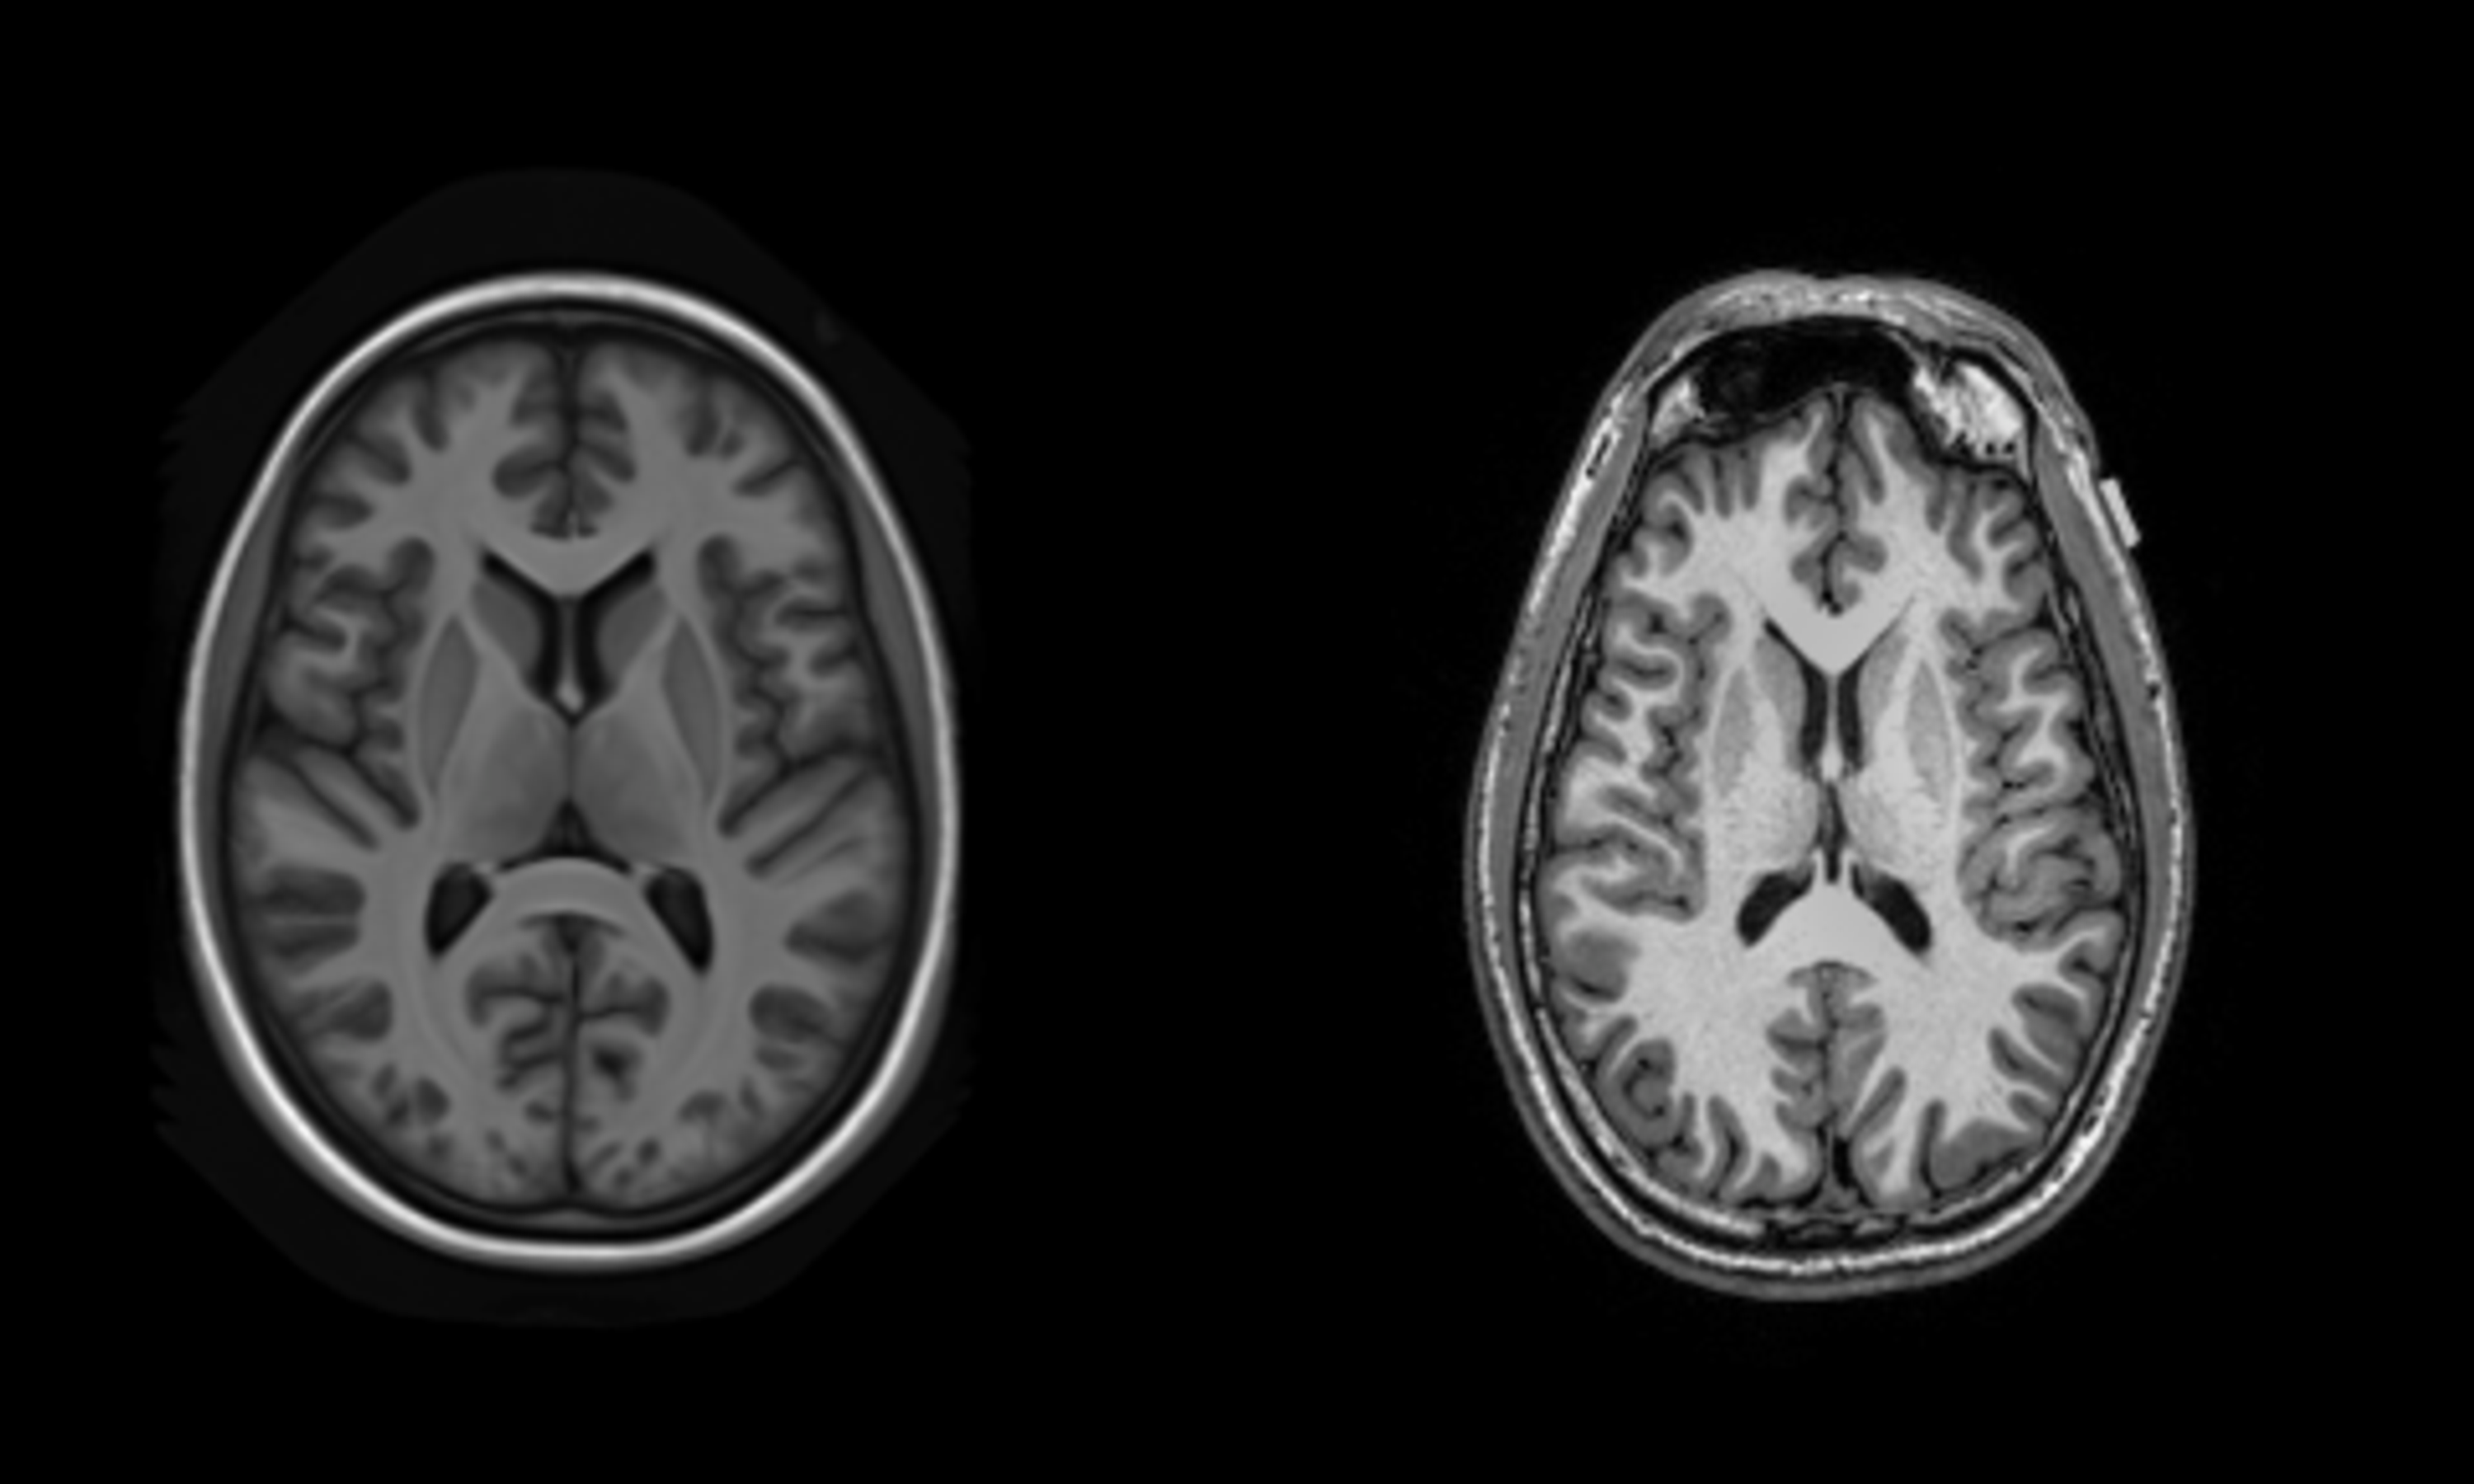
\includegraphics[width = 4.5cm]{nodots.pdf}
		        \end{center}
					  };
		    \path[->,rounded corners=0.1cm] node[format,text width=5.5cm, below of=nodots, xshift=1.1cm,yshift=2.8cm] { 
		    {\scriptsize template}
		    };
		    \path[->,rounded corners=0.1cm] node[format,text width=5.5cm, below of=nodots, xshift=3.5cm,yshift=2.8cm] { 
		    {\scriptsize subject}
		    };
}					  
\uncover<2->{    
		    \path[->,rounded corners=0.1cm] node[format,text width=5.5cm, xshift=2cm,yshift=1.5cm] (dots) { 
		        \begin{center}
       	      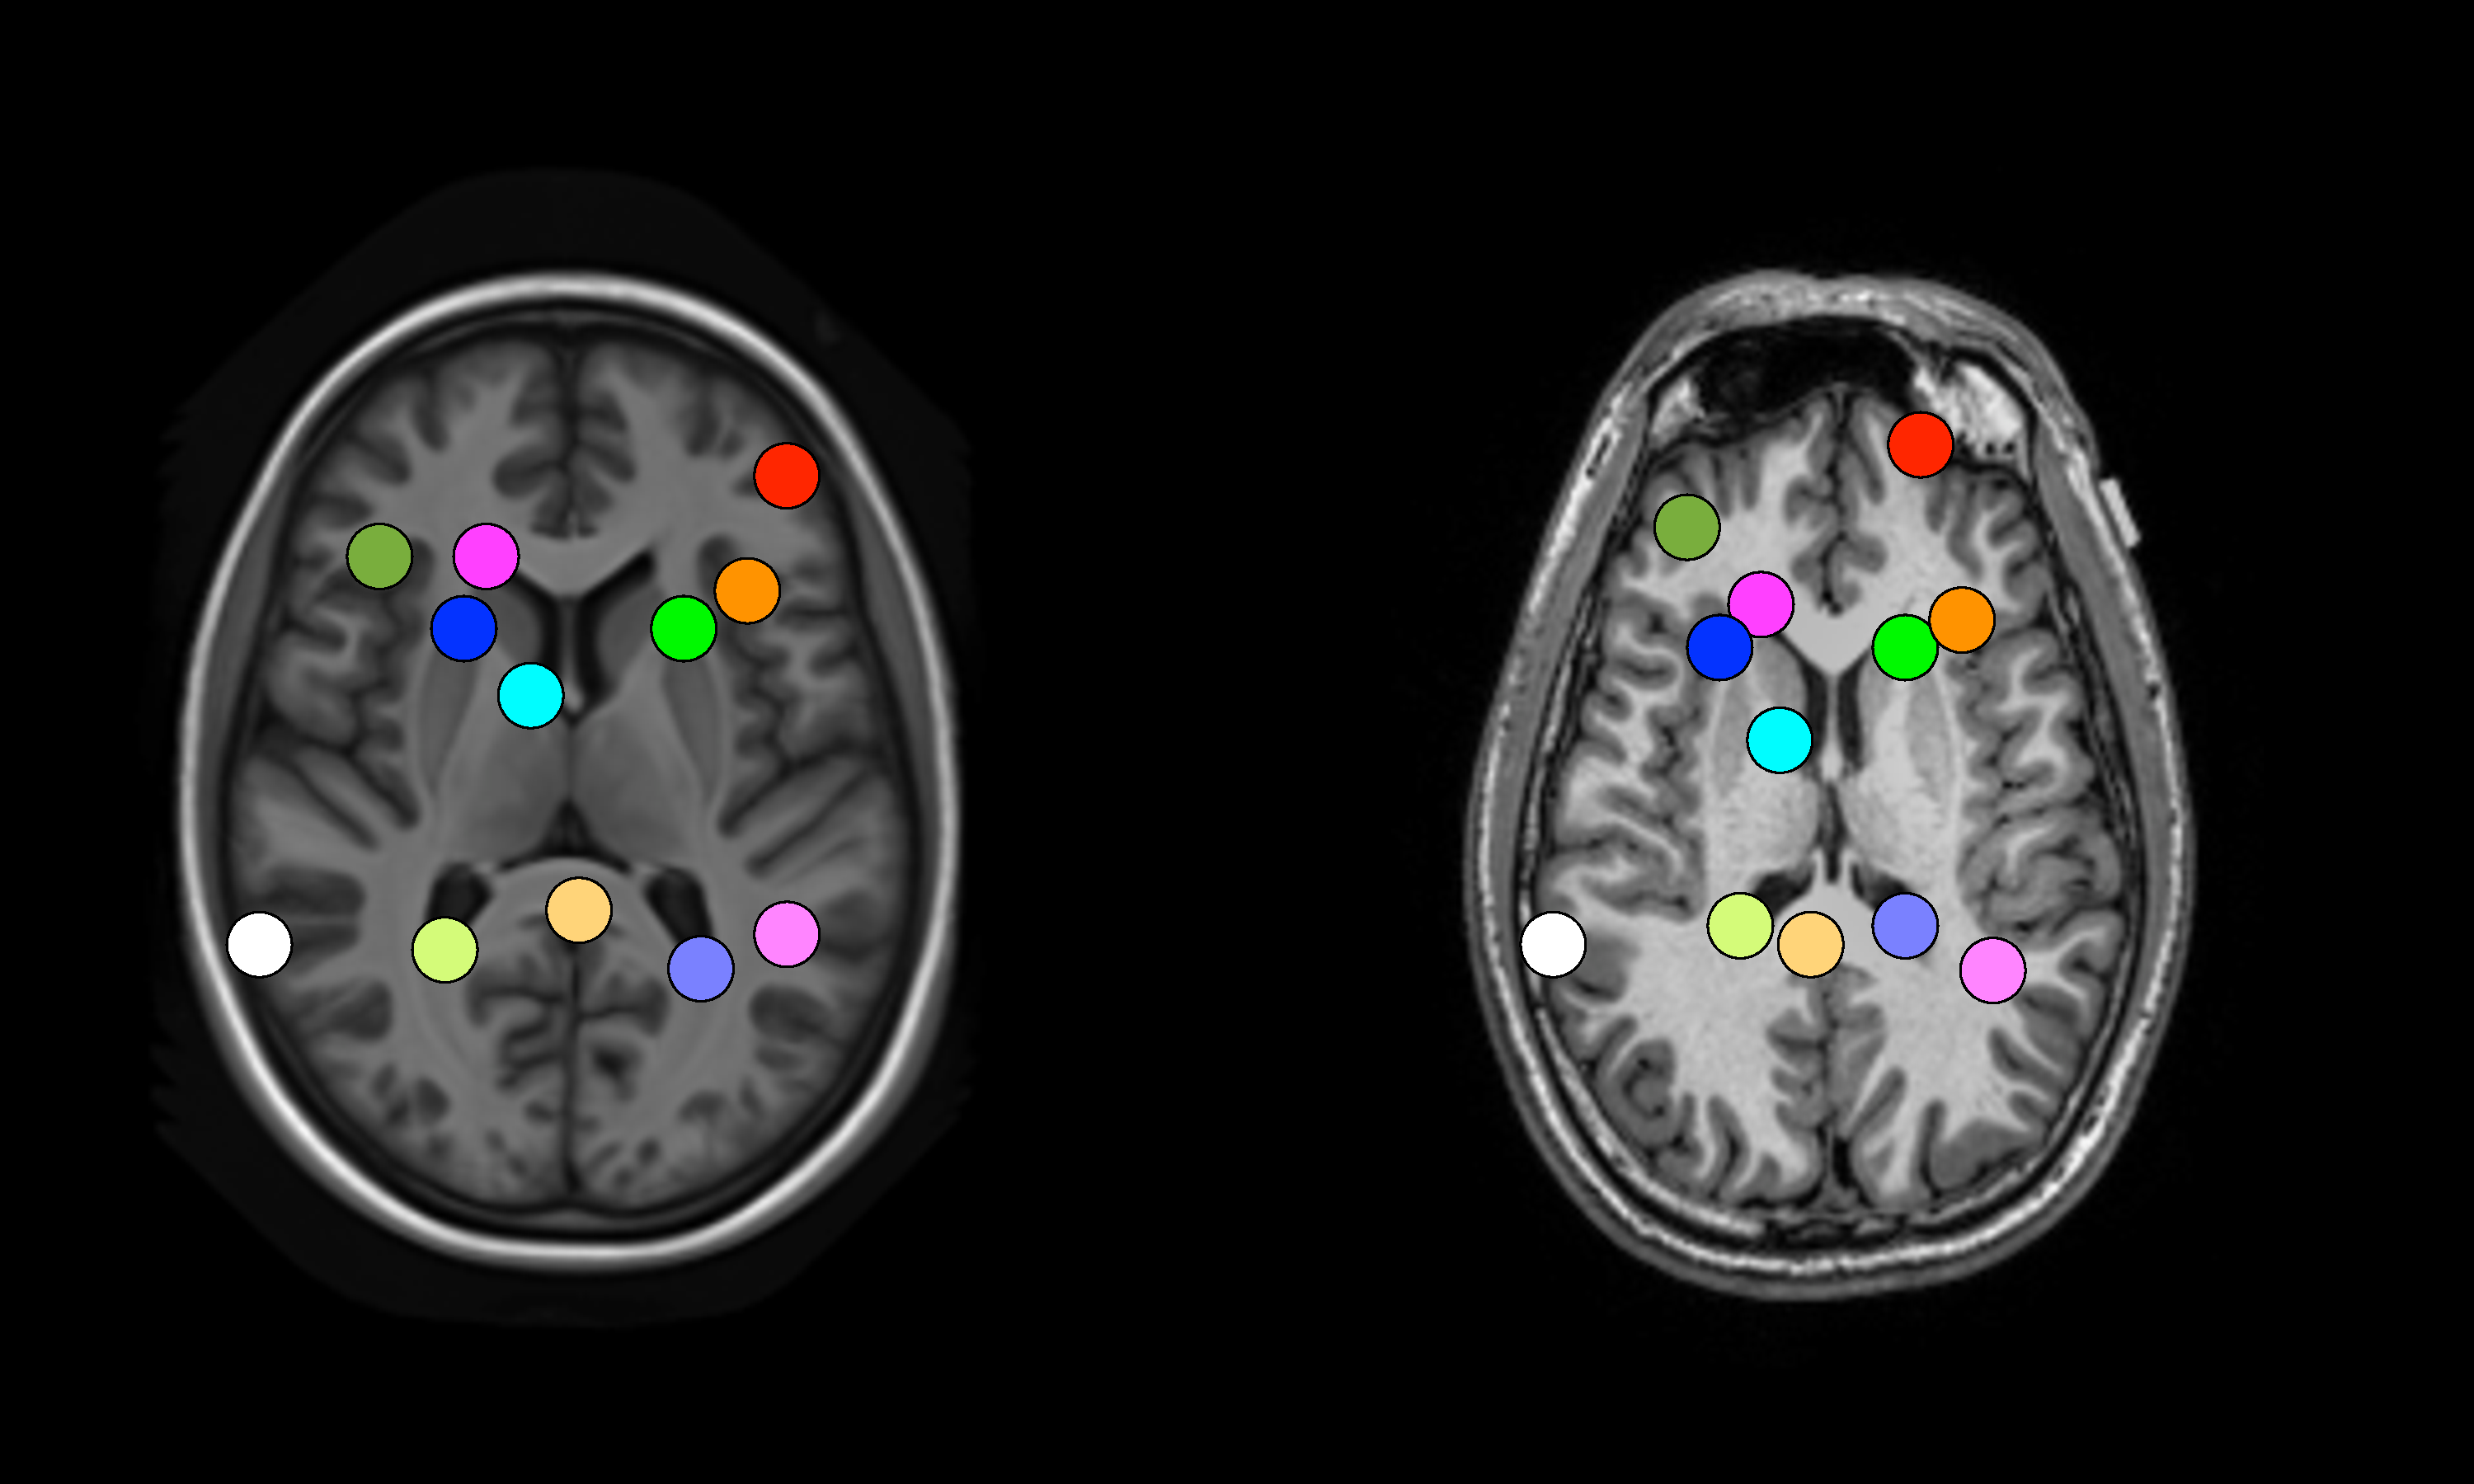
\includegraphics[width = 4.5cm]{dots.pdf}
		        \end{center}
					  };
}					  
\uncover<3->{    
		    \path[->,rounded corners=0.1cm] node[format,text width=5.5cm, text height=-0.3cm, below of = dots] (pair) { 
		        \begin{center}
		          \begin{tabular}{c}
         	      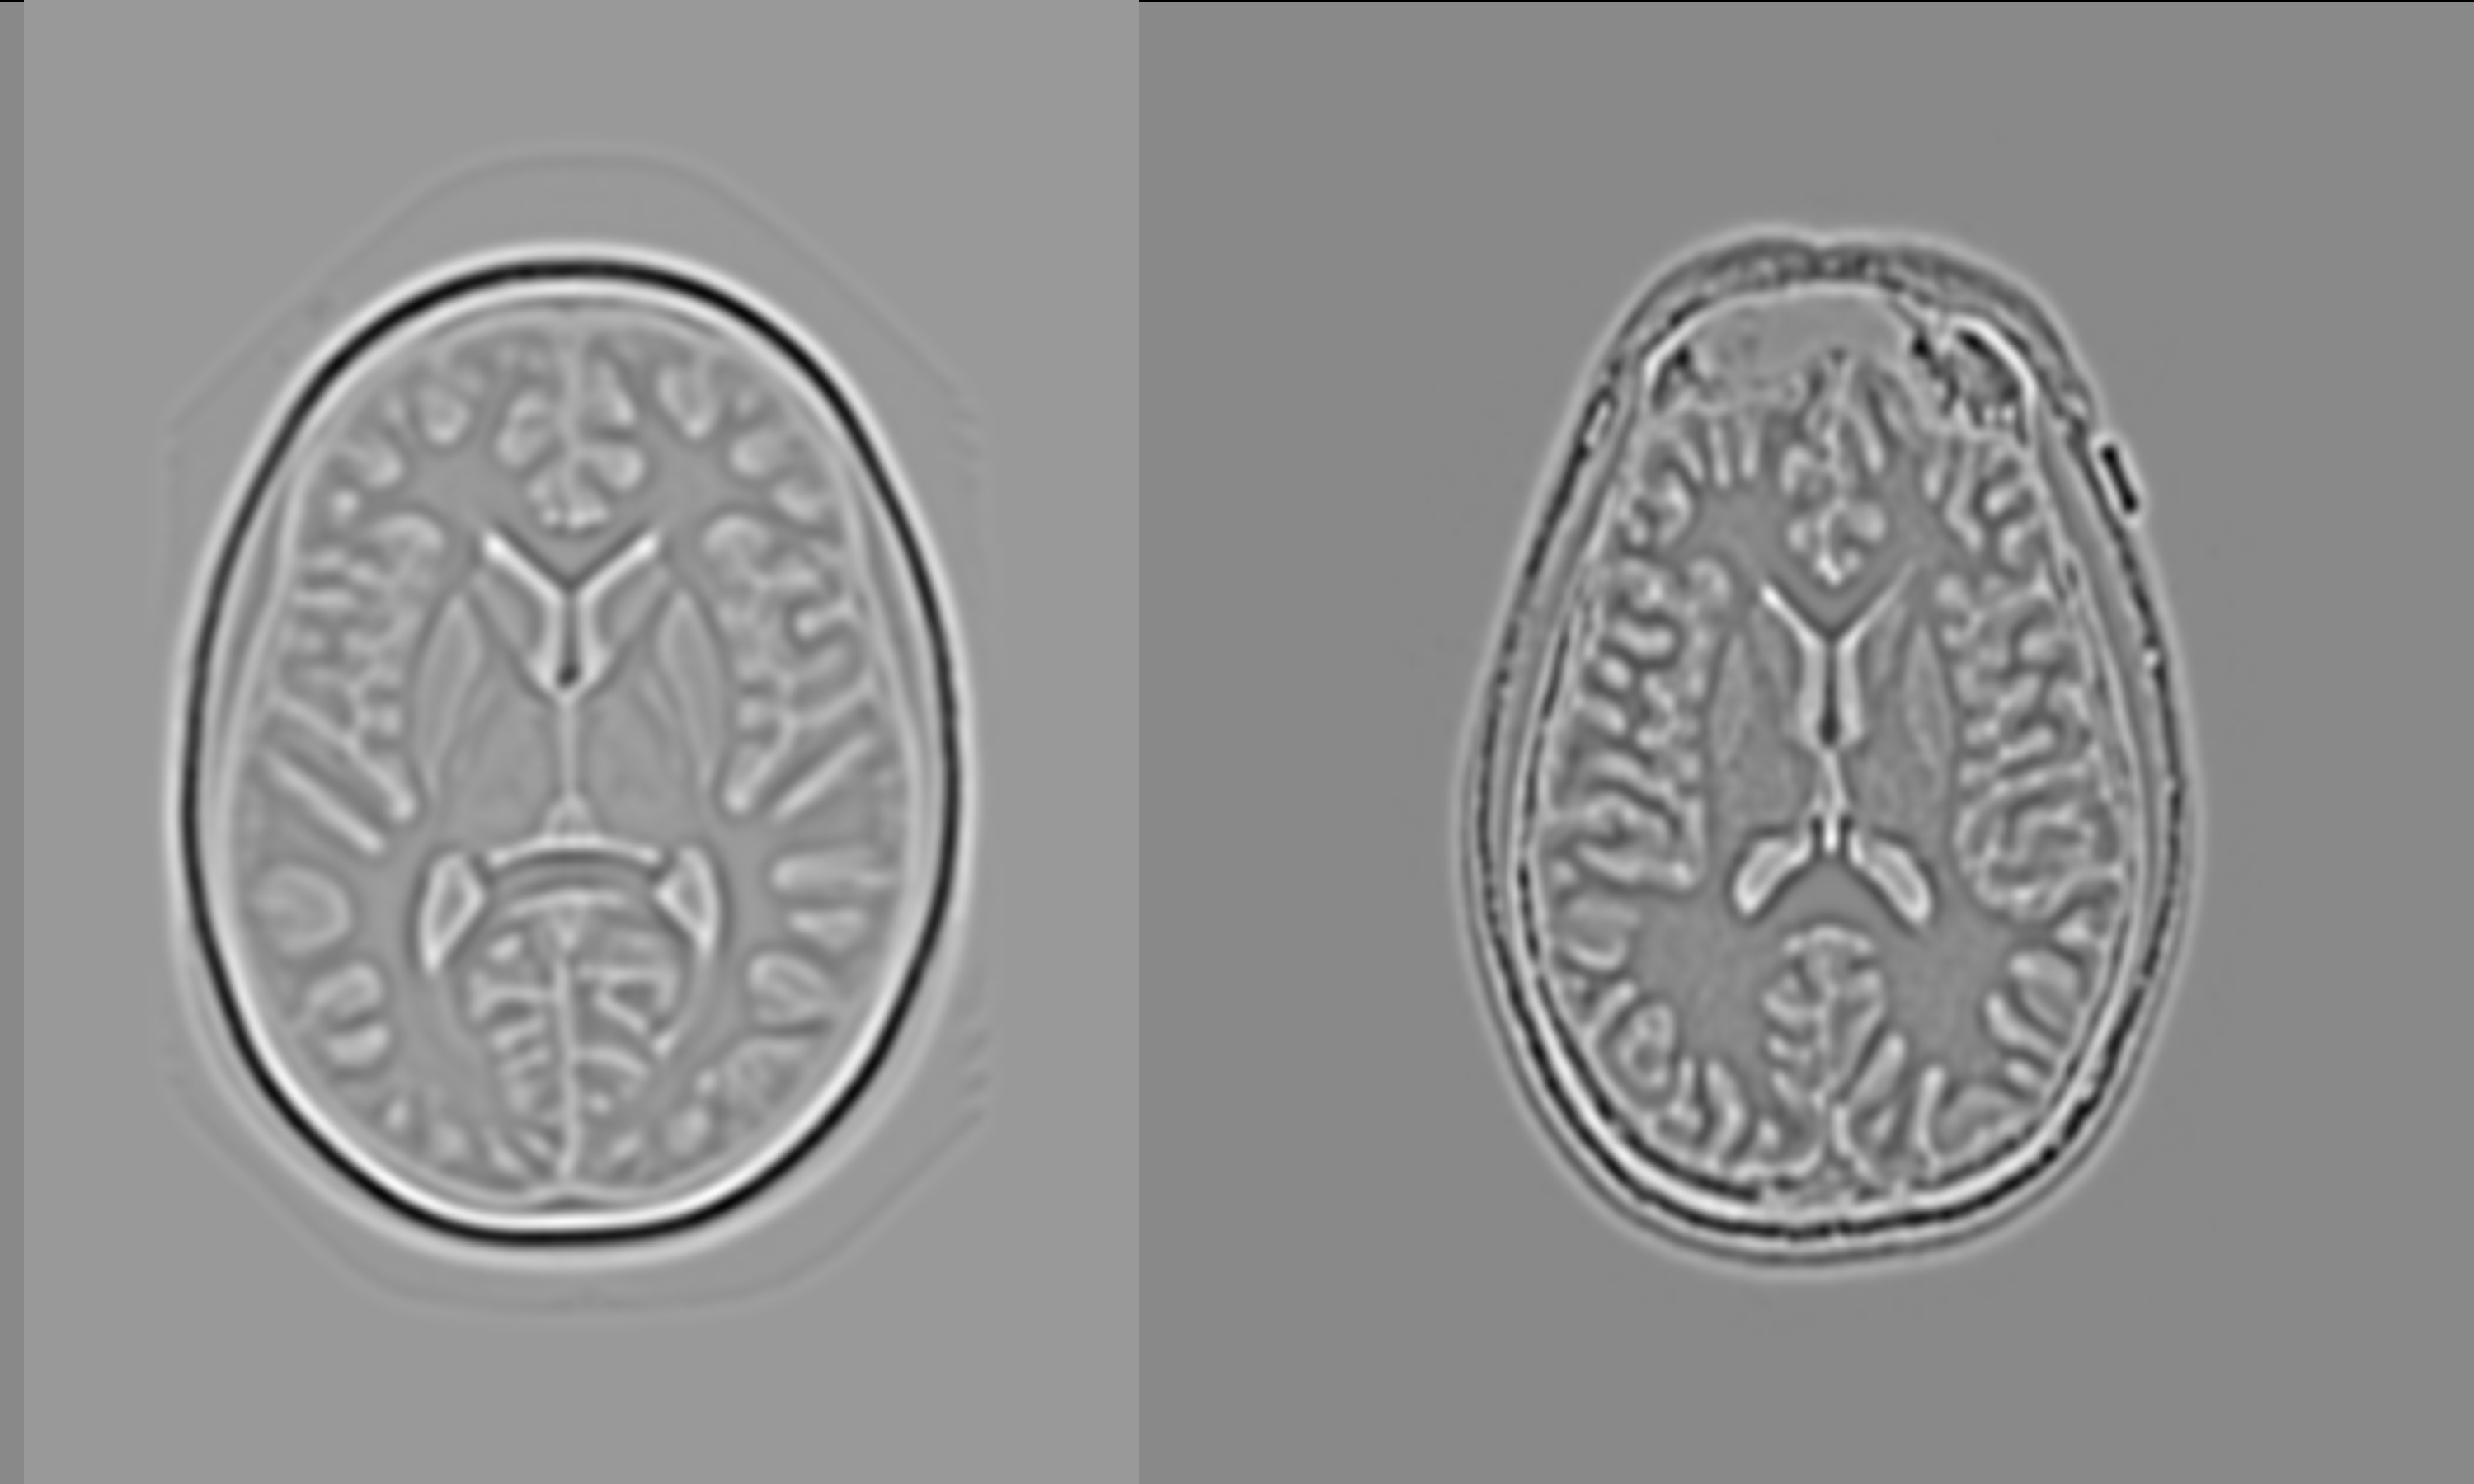
\includegraphics[width = 2.5cm]{laplacian.pdf} \\
         	      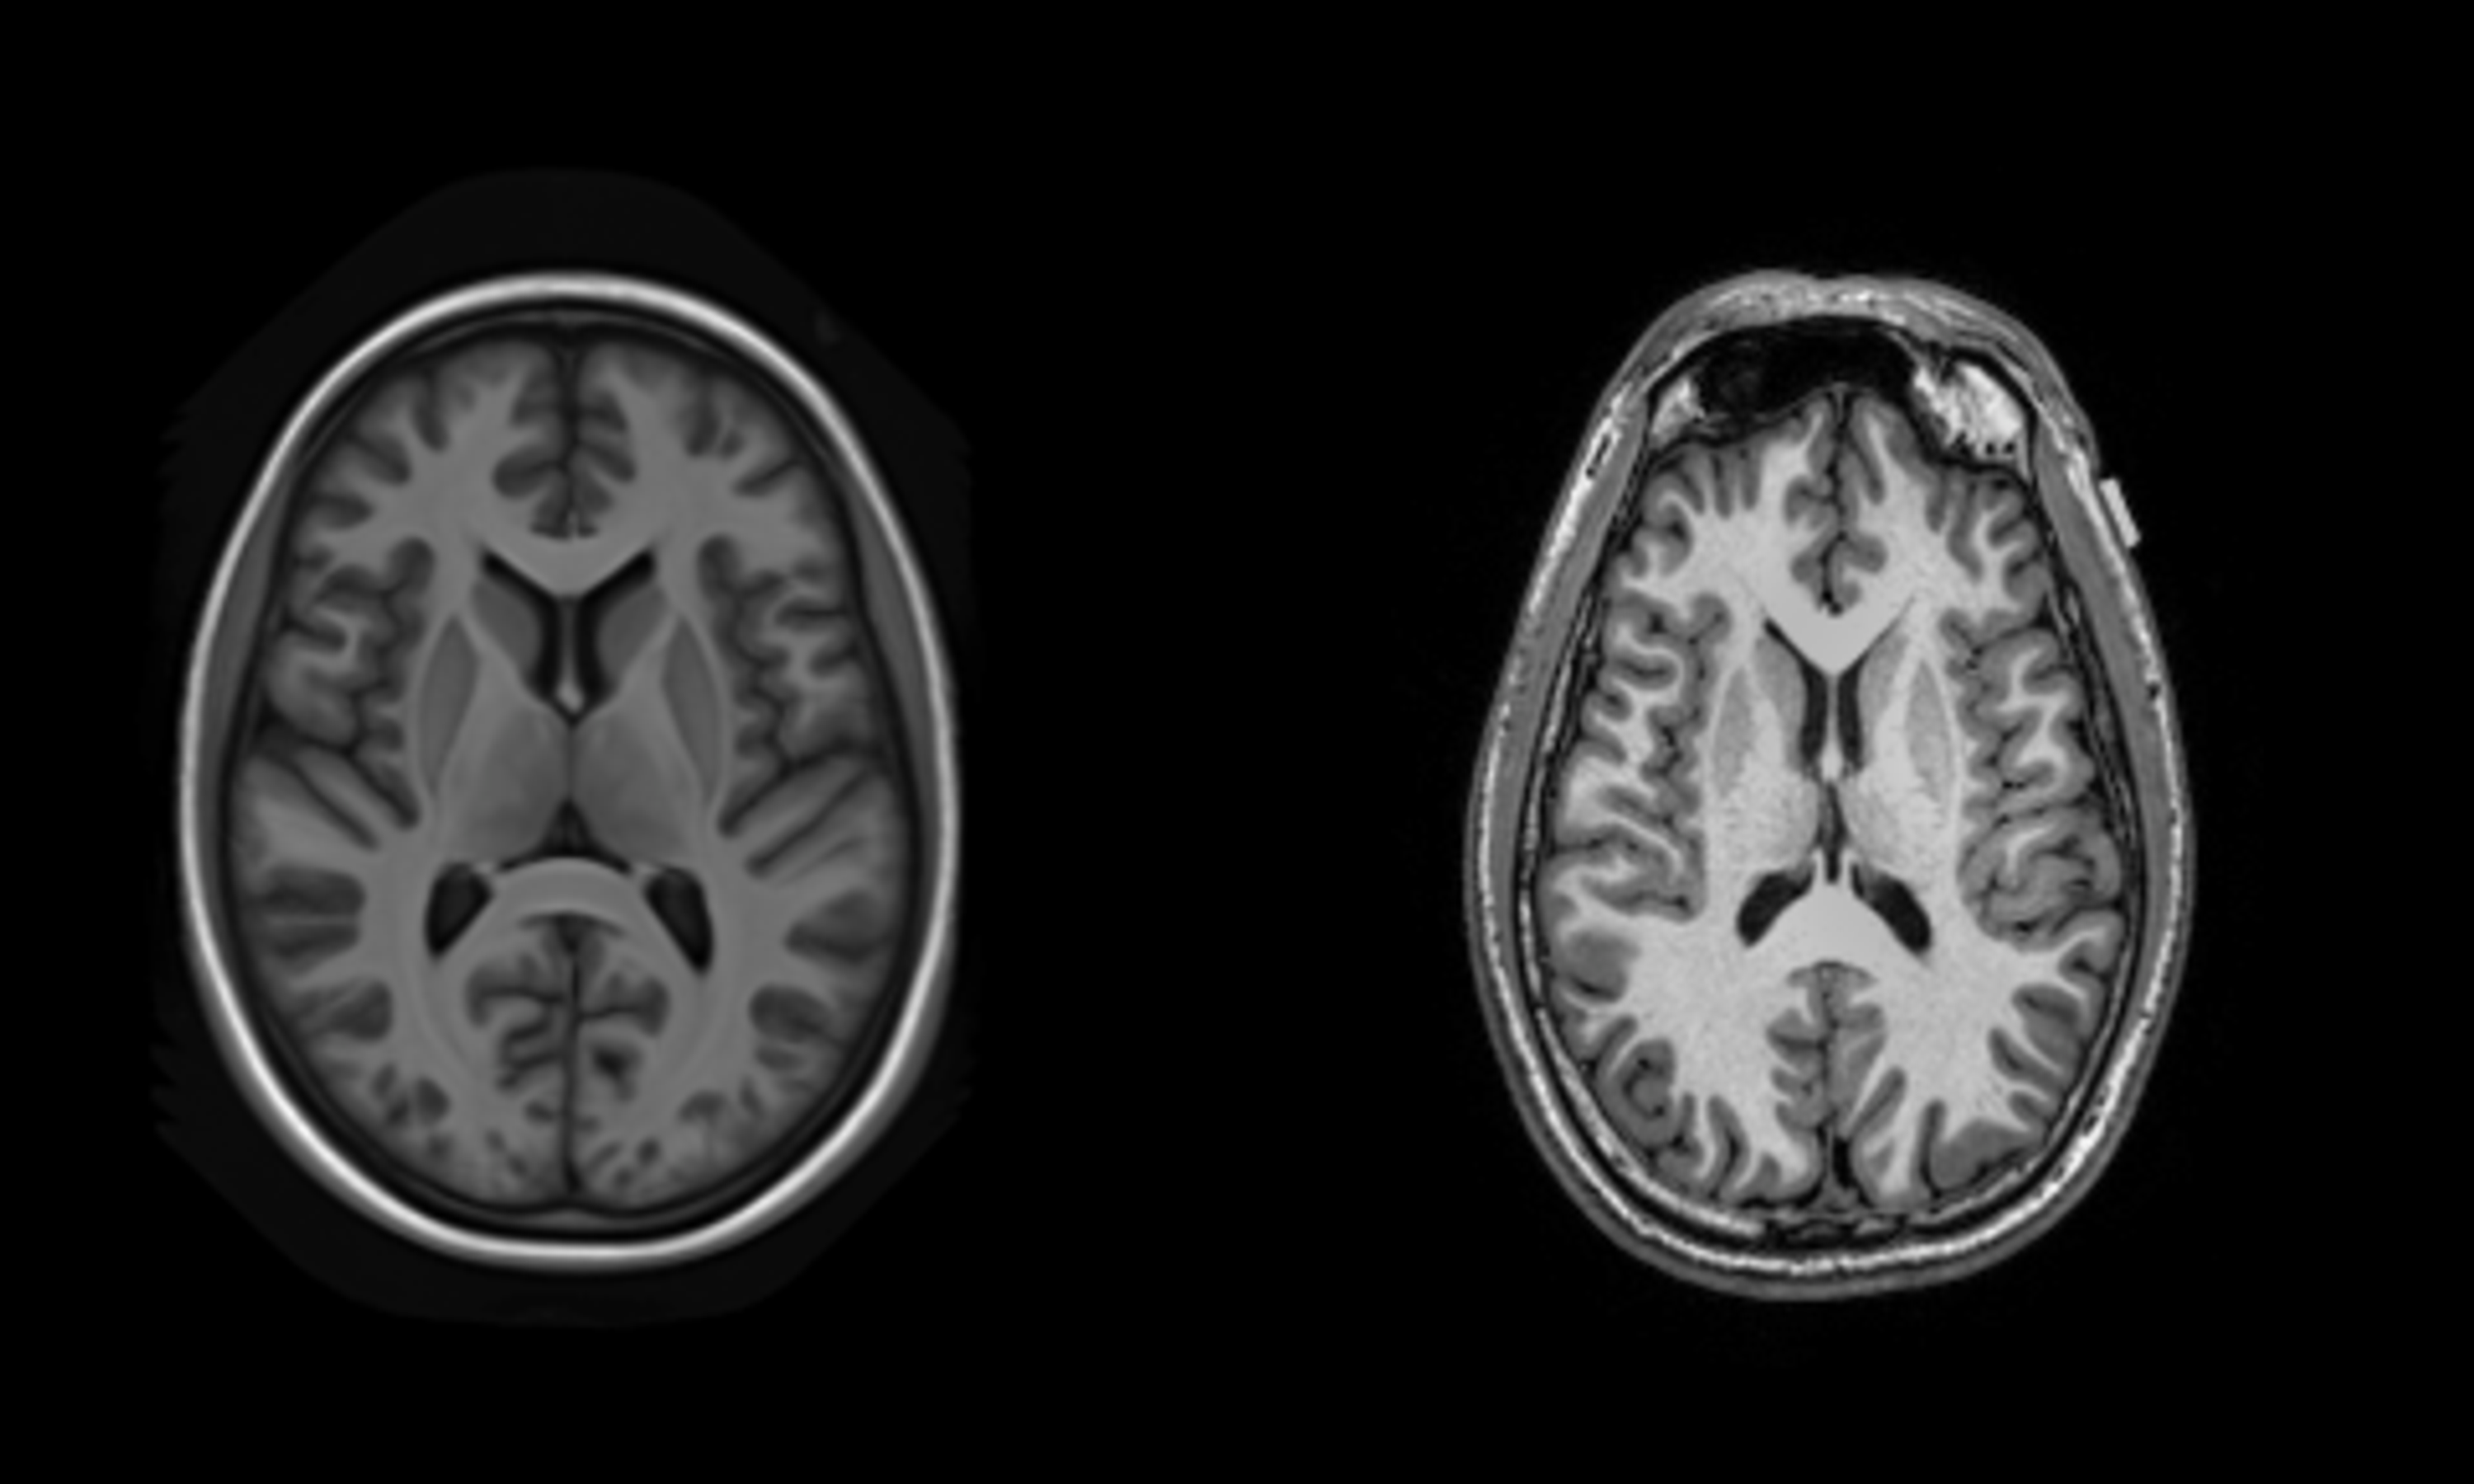
\includegraphics[width = 2.5cm]{nodots.pdf}
	            \end{tabular}
		        \end{center}
					  };
        \path[draw, -latex'] (nodots) -- node{\scriptsize Affine init.} (pair);			  
}					  

\uncover<4->{    
    \path[->,rounded corners=0.1cm] node[format,text width=5.5cm, right of = dots, xshift=2cm, yshift=-2cm] (fails) { 
        \begin{center}
    	      {Extraction failures} \\
     \vspace{0.5cm}
   \begin{tabular}{cc}
     \begin{sideways}\texttt{IXI\_191}\end{sideways} & 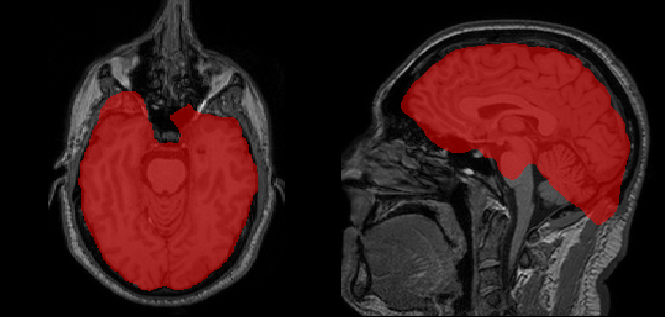
\includegraphics[width=4cm]{IXI191_failure.png} \\
     \begin{sideways}\texttt{IXI\_370}\end{sideways} & 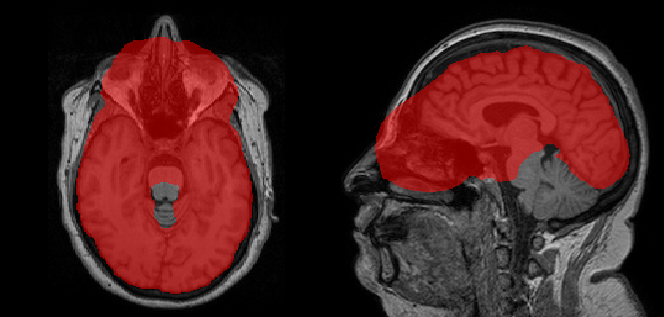
\includegraphics[width=4cm]{IXI370_failure.png} \\
     \begin{sideways}\texttt{IXI\_594}\end{sideways} & 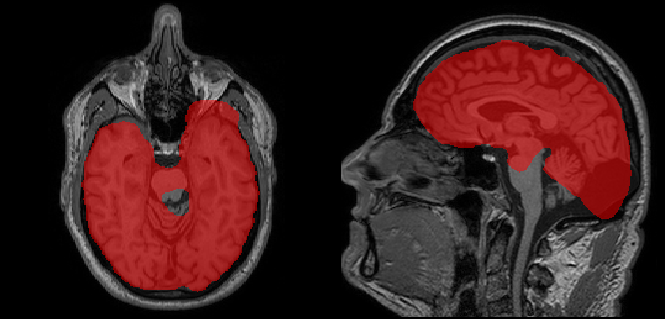
\includegraphics[width=4cm]{IXI594_failure.png} 
   \end{tabular}
        \end{center}

			  };
}

\end{tikzpicture}

\end{frame}

%%%%%%%%%%%%%%%%%%%%%%%%%%%%%
%%  N4 Atropos brain segmentation
%%%%%%%%%%%%%%%%%%%%%%%%%%%%%

\begin{frame}{N4 $\leftrightarrow$ Atropos}

\tikzstyle{format} = []

\begin{center}
\begin{tikzpicture}[node distance=4cm, auto,>=latex', thin]
  % We need to set at bounding box first. Otherwise the diagram
 	% will change position for each frame.
  \path[use as bounding box] (-1,0) rectangle (10,0);
 
\uncover<1->{ 
  \path[->,rounded corners=0.1cm] node[format,text width=1.75cm, xshift = -0.35cm] (extraction) { 
      \begin{center}
          \begin{tabular}{cc}
    	        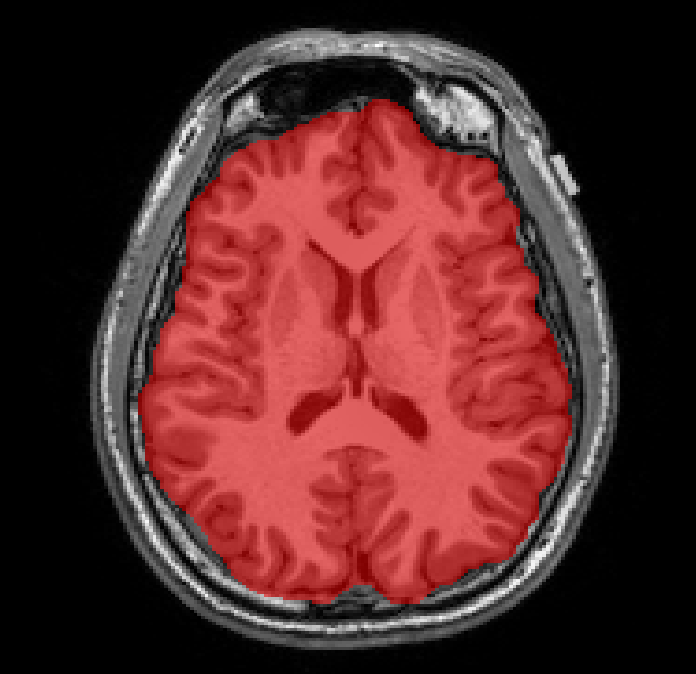
\includegraphics[width = 1.75cm]{extraction.png} &
    	        
\includegraphics[width = 1.75cm]{weightmask.png} \\
	           {\scriptsize brain mask} & 
	           {\scriptsize weight mask}
	           \end{tabular}
      \end{center}
	};
}	
\uncover<2->{ 
  \path[->,rounded corners=0.1cm] 
    node[format,text width=1.75cm, yshift=2cm, xshift=1.75cm,right of=extraction] (n4) { 
      \begin{center}
        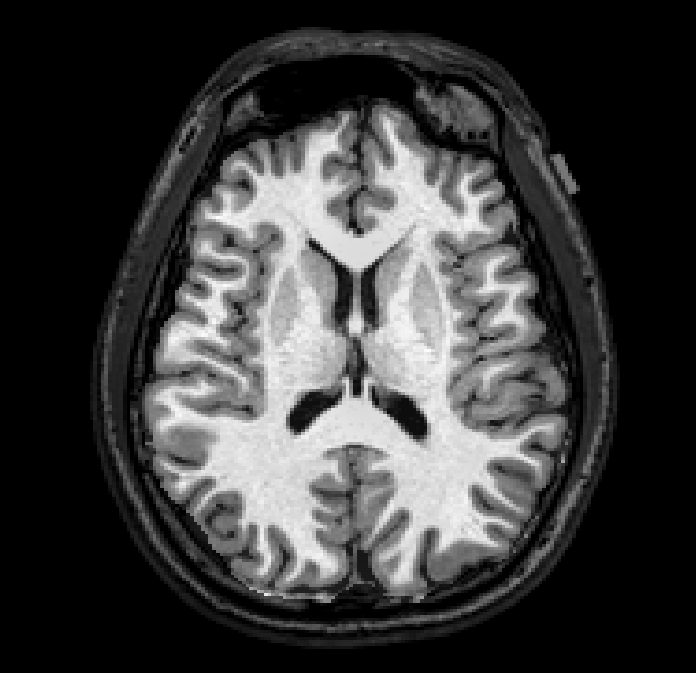
\includegraphics[width = 1.75cm]{n4.png} \\
        {\scriptsize N4}
      \end{center}
	};
  \path[->,thick] (extraction.45) edge [out=45, in=180] (n4.180);			  
}  
\uncover<3->{ 
  \path[->,rounded corners=0.1cm] 
    node[format,text width=1.75cm, yshift=-2cm, right of=n4] (atropos) { 
      \begin{center}
        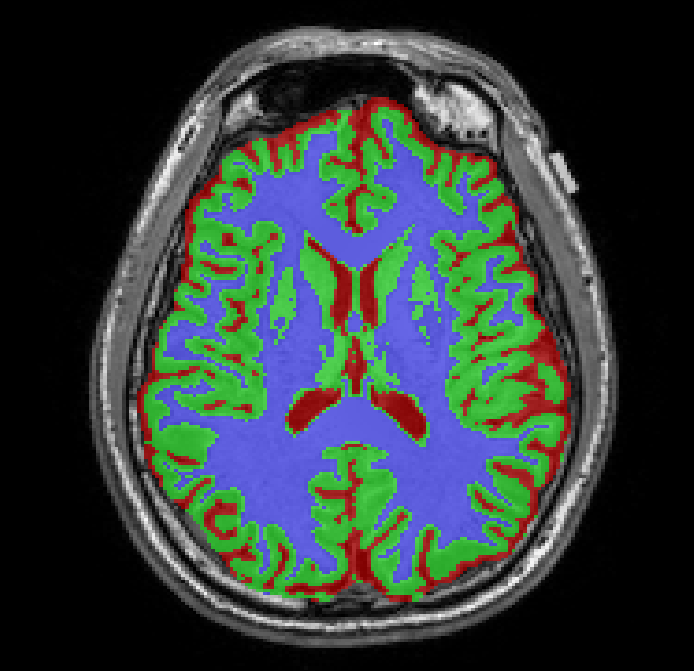
\includegraphics[width = 1.75cm]{segmentation.png} \\
	        {\scriptsize Atropos}
      \end{center}
	};
  \path[->,thick] (n4.0) edge [out=0, in=135] (atropos.90);			  
}

\uncover<4->{ 
  \path[->,rounded corners=0.1cm] 
    node[format,text width=2.5cm, below of=n4] (conv) { 
      \begin{center}
        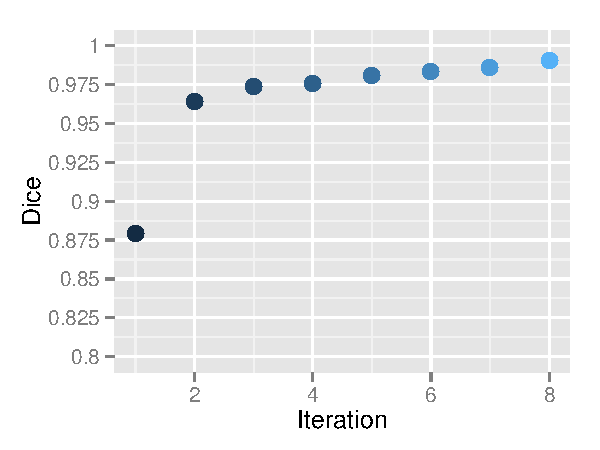
\includegraphics[width = 2.5cm]{convergence.pdf} \\
	        {\scriptsize Convergence?}
      \end{center}
	};
  \path[->,thick] (atropos.-90) edge [out=-135, in=0] (conv.0);			  
}	

\uncover<5->{ 
  \path[->,thick] (conv.180) edge [out=180, in=-45] (extraction.-45);			  
  \draw[->,thick,dashed] (atropos.180) -- node {\scriptsize update weight mask} ([xshift=1.75cm]extraction.0);			  
}  
     
\end{tikzpicture}
\end{center}

\end{frame}

%%%%%%%%%%%%%%%%%%%%%%%%%%%%%
%%  DiReCT
%%%%%%%%%%%%%%%%%%%%%%%%%%%%%

%\begin{frame}{DiReCT}
%
%\end{frame}


%%%%%%%%%%%%%%%%%%%%%%%%%%%%%
%%  IXI Thickness
%%%%%%%%%%%%%%%%%%%%%%%%%%%%%

\begin{frame}{$\texttt{thickness} \sim 1 + \texttt{age} + \texttt{I(age\^{}2)}$}

\tikzstyle{format} = []

\begin{center}
\begin{tikzpicture}[node distance=4cm, auto,>=latex', thin]
    % We need to set at bounding box first. Otherwise the diagram
    % will change position for each frame.
    \path[use as bounding box] (-1,0) rectangle (10,0);

\uncover<1->{    
    \path[->,rounded corners=0.1cm] node[format,text width=5.5cm,xshift=1.5cm,yshift=-0.5cm ] (nirep) { 
        \begin{center}
			  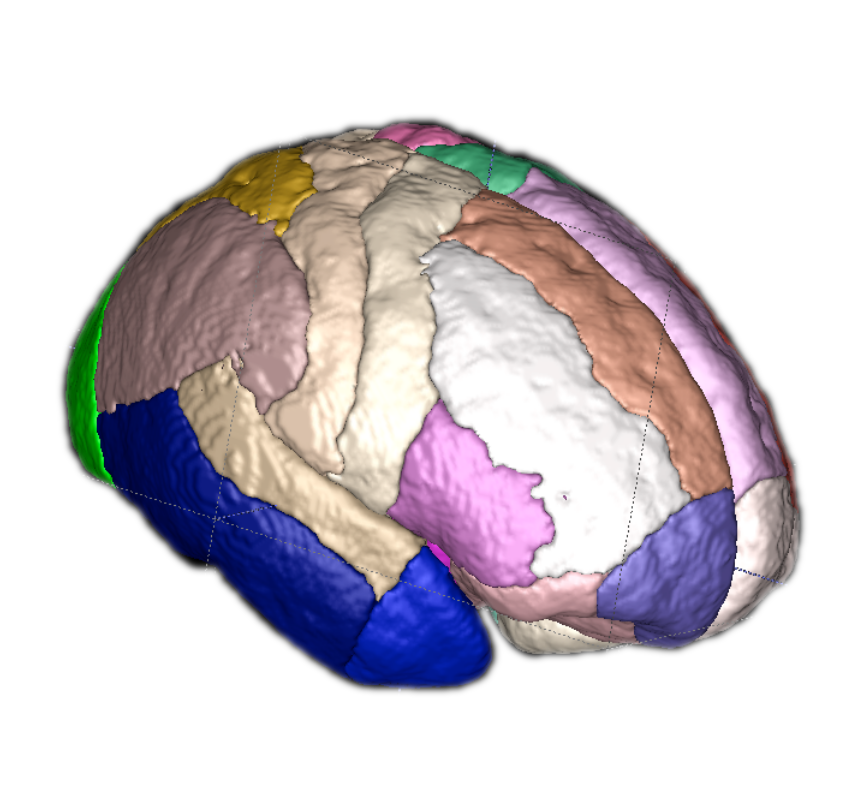
\includegraphics[width=5.5cm]{NIREPLabels.png} \\
        \end{center}
			  };
}			  
\uncover<2->{    
    \path[->,rounded corners=0.1cm] 
      node[format, right of=nirep, xshift=2.25cm, yshift=1.85cm,text width=4.5cm] (rp) {
        \begin{center}
			  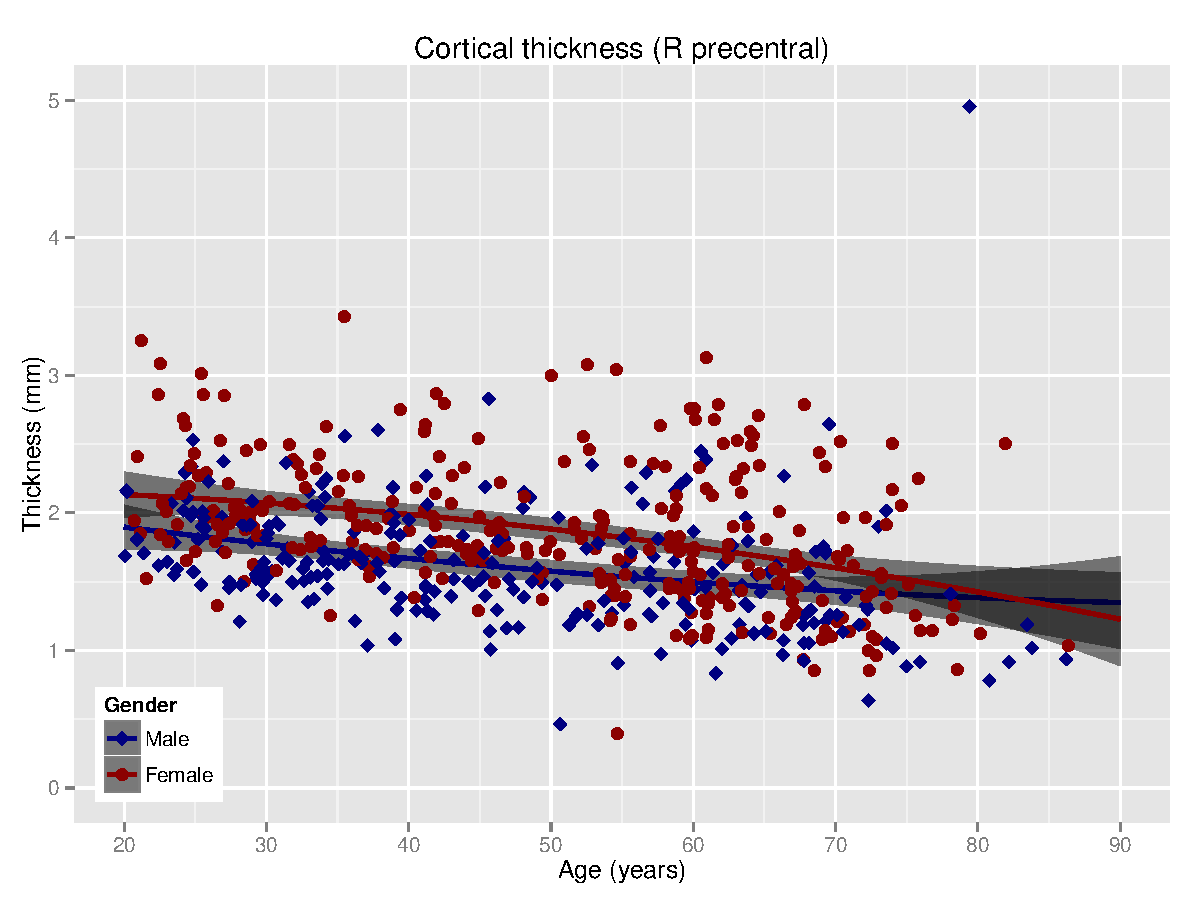
\includegraphics[width=4.5cm]{yylabel26_results.pdf}
        \end{center}
			  };
    \path[->,thick, color = yellow] (rp.west) edge [out= 180, in= 90] (1.25,0);			  
}			  
\uncover<3->{    
    \path[->,rounded corners=0.1cm] 
      node[format, right of=nirep, xshift=2.25cm, yshift=-1.85cm,text width=4.5cm] (rt) {
        \begin{center}
			  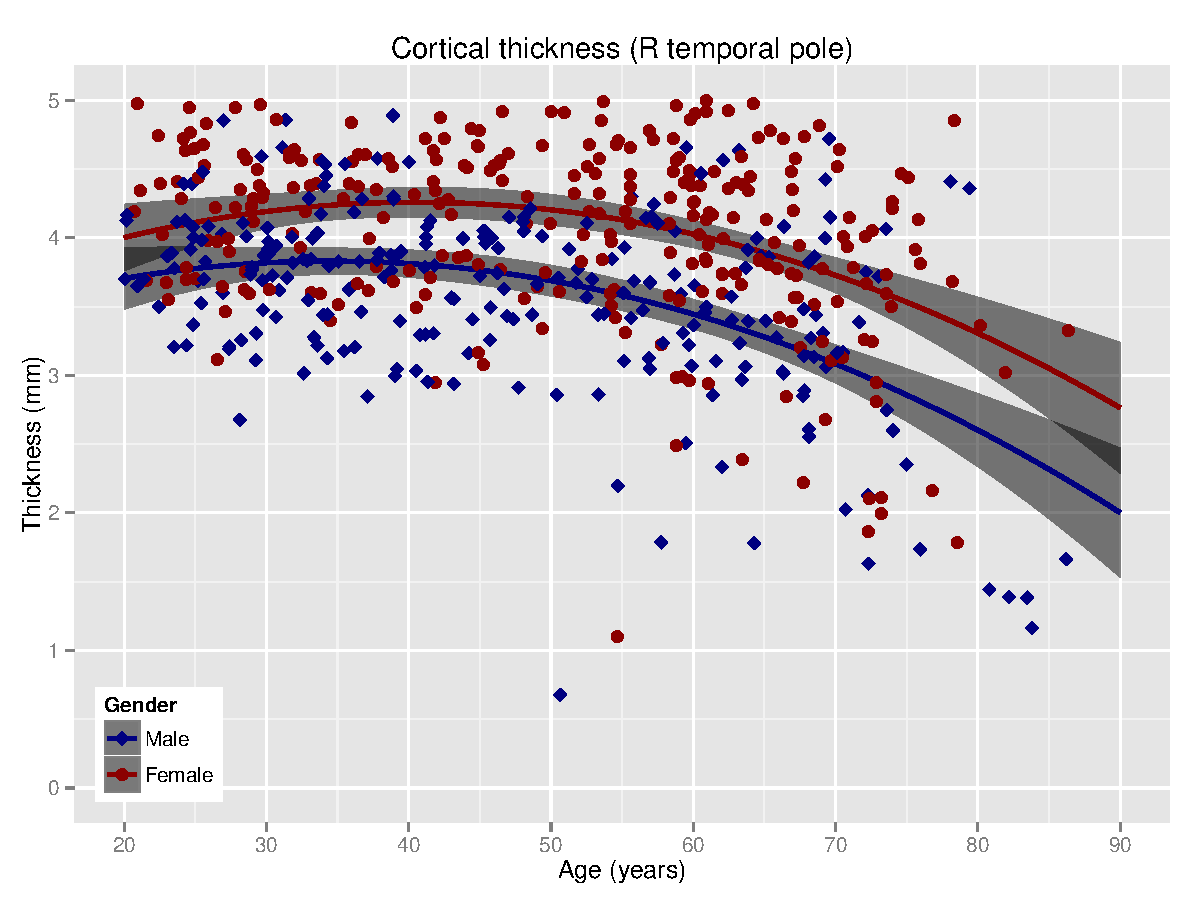
\includegraphics[width=4.5cm]{yylabel8_results.pdf} \\
        \end{center}
			  };
    \path[->,thick, color = yellow] (rt.west) edge [out= 180, in= 270] (1.4,-2.);
}			  
\end{tikzpicture}

%\begin{tikzpicture}
%  \tikz[overlay]\path[->,thick, color = yellow] (rp.west) edge [out= 180, in= 90] (-2.6,5);
%  \tikz[overlay]\path[->,thick, color = yellow] (rt.west) edge [out= 180, in= 270] (-2.5,2.75);
%\end{tikzpicture}

\end{center}

\end{frame}

%%%%%%%%%%%%%%%%%%%%%%%%%%%%%
%%  Closing slide
%%%%%%%%%%%%%%%%%%%%%%%%%%%%%

\begin{frame}{}


\begin{tikzpicture}[node distance=1cm, auto,>=latex', thin]
    % We need to set at bounding box first. Otherwise the diagram
    % will change position for each frame.
    \path[->,rounded corners=0.1cm] node[text width=2cm,xshift=-2cm] (ants) { 
        \begin{center}
			  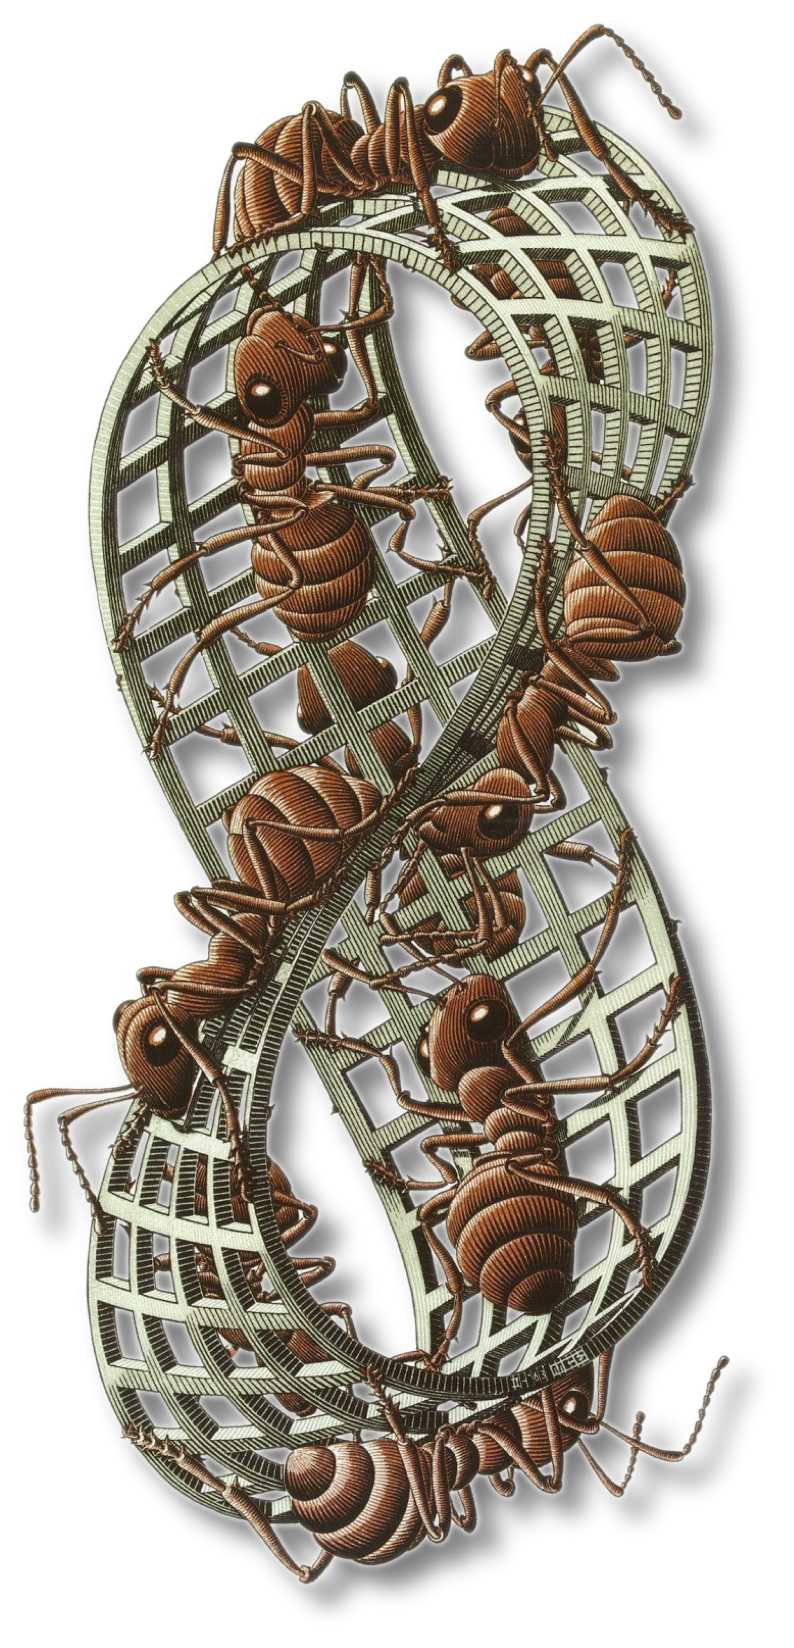
\includegraphics[width=3.5cm]{ants2.png} \\
        \end{center}
			  };
    \path[->,rounded corners=0.1cm] node[text width=6.5cm, xshift=5.5cm, right of=ants] { 
        \begin{center}
        \begin{block}{Further information}
        \begin{itemize}
          \item \url{http://www.itk.org}
          \item \url{http://www.picsl.upenn.edu/ANTs}
        \end{itemize}
        \end{block}
        \end{center}
			  };
			  
\end{tikzpicture}
\end{frame}

\end{document}